\documentclass[12pt]{article}

% ===== Packages =====
\usepackage[margin=1in]{geometry}
\usepackage{setspace}
\usepackage{graphicx}
\usepackage{booktabs}
\usepackage{amsmath}
\usepackage{caption}
\usepackage{float}
\usepackage{times}
\usepackage[hidelinks]{hyperref}
\usepackage{microtype}
\usepackage{indentfirst} % indent the first paragraph of every section

\captionsetup{font=small,labelfont=bf}
\setlength{\parindent}{0.4in}
\graphicspath{{illustration/}}

% Hanging-indent helper for the APA reference list
\newcommand{\refitem}[1]{\par\noindent\hangindent=0.5in\hangafter=1 #1\vspace{6pt}}

\begin{document}

% =====================================================================
% TITLE PAGE
% =====================================================================

\begin{titlepage}
\centering
\vspace*{2.5cm}

{\Large\bfseries Monetary Tightening and the Affordability Gap\\[0.3em]
Across Canadian Housing Markets\par}

\vspace{0.6cm}
{\large Final Paper\par}

\vspace{3cm}

\vspace{0.4cm}
Mai Tran

\vspace{0.4cm}
Wilfrid Laurier University

\vspace{0.2cm}
EC481-J: Research Paper and Seminar

\vspace{0.2cm}
Instructor: Dr. David Ros\'e

\vspace{0.2cm}
August 10, 2026

\vfill
\noindent\rule{\textwidth}{0.4pt}\\[0.3em]
{\footnotesize The generative AI assistant Claude (Anthropic) was used to help format this report in \LaTeX, refine the structure and exposition, and check the internal consistency and accuracy of the theoretical and econometric arguments. All research design, data construction, estimation, and interpretation are the author's own, and all outputs were verified by the author against the underlying Stata log.\par}

\end{titlepage}

\doublespacing
\setcounter{page}{1}

% =====================================================================
\section{Introduction}
% =====================================================================

The post-2022 monetary tightening cycle in Canada created a direct conflict between inflation control and housing affordability. Beginning in March 2022, the Bank of Canada raised its policy rate from near zero to 4.25\% by December 2022 (Bank of Canada, 2022a, 2022b, 2022c). Higher policy rates increased mortgage borrowing costs and, through the regulatory mortgage stress test, reduced the maximum price that households could finance. According to the Office of the Superintendent of Financial Institutions (OSFI) rule, borrowers must qualify at either two percentage points above their contract rate or a 5.25\% floor, whichever is higher. Consequently, the 2022–2023 increase in posted rates resulted in a sharper contraction in the price at which households could be approved for financing (OSFI, 2025). Because affordability consistently ranks among the most significant economic concerns for Canadian households, the distributional consequences of national rate decisions are of broad public importance.

Major urban markets were already significantly stretched prior to the onset of monetary tightening. According to the Parliamentary Budget Officer's (PBO) borrowing-capacity estimates, several large cities became "de-linked" from household borrowing capacity well before the pandemic, and affordability has since diverged across markets rather than converged (PBO, 2022, 2025). This study investigates whether the post-2022 contraction in qualified purchasing power was distributed evenly or concentrated in markets that were already stretched. The central research question is: \emph{did the post-2022 rise in mortgage qualifying rates widen the gap between home prices and mortgage-qualified purchasing capacity more in markets that were already expensive relative to local income before 2022?}

To address this question, a panel of 36 Canadian census metropolitan areas (CMAs) covering 2016–2023 is assembled. A market-level affordability gap is constructed as the logarithmic difference between the benchmark home price and the maximum price a median-income census family could qualify to finance under the OSFI rule. Each market's pre-2022 exposure is defined as its standardized average price-to-income ratio over 2016–2021. A continuous-treatment difference-in-differences model is estimated, in which the qualifying rate is interacted with this exposure, and market and year fixed effects are included.

The central finding is a precisely estimated near-zero effect. The exposure interaction is small, negative, and statistically insignificant ($\hat{\beta}=-0.015$, $p=0.26$). This effect becomes negligible once Toronto and Vancouver or all of British Columbia are excluded, and a wild cluster bootstrap, which is appropriate given the small number of clusters, yields an even larger $p$-value of $0.39$. The estimate is interpreted as correlational rather than causal, with an important caveat: because pre-exposure is itself a pre-period price-to-income ratio and the outcome is closely related to that same ratio once year effects absorb the national rate, the specification risks capturing a mechanical mean-reversion relationship rather than a behavioral response to tightening. The contribution of this study is both methodological and substantive. Instead of presenting a potentially fragile positive result, the analysis explains why identifying a differential-exposure effect in Canadian data during this period is challenging. Specifically, two offsetting economic channels, a dominant common shock, and a mechanical mean-reversion issue complicate identification. The only specification that produces significant results does so by violating the parallel trends assumption. The main practical implication is a clear distributional finding: the 2022 to 2023 tightening of monetary policy reduced mortgage access by a similar magnitude in both expensive and affordable markets, indicating that the impact was national rather than concentrated in the most stretched cities.




% =====================================================================
\section{Literature Review}
% =====================================================================

This analysis is informed by three strands of research. The first strand investigates regional heterogeneity in monetary transmission. Beraja, Fuster, Hurst, and Vavra (2019), in the Quarterly Journal of Economics, combine loan-level mortgage records with a heterogeneous-household model to demonstrate that regional differences in housing equity influence households' responses to interest-rate changes. Although their analysis focuses on refinancing following rate cuts, the present study emphasizes qualification under rate increases, while maintaining the core insight that local housing-market conditions mediate the effects of a common national shock. Rao and Wang (2026), in a Bank of Canada staff analytical paper, extend this logic to Canadian prices, estimating that mortgage-rate movements affect house prices and rents unevenly across cities. This uneven transmission helps explain why the affordability gap may not respond uniformly to a national rate path. Both studies inform the exposure design: if transmission is heterogeneous, then pre-existing exposure is the appropriate dimension along which to examine differential effects.

The second strand is the applied borrowing-capacity approach to affordability developed by the PBO (2022, 2025), which builds on the International Monetary Fund's framework for assessing Canadian house prices (IMF, 2019). The PBO defines the affordability gap as the difference between the actual benchmark price and the price a household of a given income can support. This analysis adopts the borrowing-capacity conception of affordability, but implements it through the OSFI qualifying rule rather than a payment-affordability threshold. Consequently, the gap measures access to mortgage approval instead of payment burden. This approach extends the PBO framework by converting it into a market-year panel outcome that can be interacted with the qualifying-rate path.

The third strand is methodological, providing both the estimator and the inference procedure used in this analysis. The design employs a continuous dose-response difference-in-differences estimator, where a continuously varying treatment intensity (the qualifying rate) interacts with continuous cross-sectional exposure. The relevant theory is presented by Callaway, Goodman-Bacon, and Sant'Anna (2024) in a National Bureau of Economic Research working paper, who formalize the assumptions under which continuous-treatment designs yield interpretable causal parameters. The key requirement is a strong version of parallel trends holding across the treatment support.This is tested directly through the event study and, in the extension, is found to fail. For inference, a primary concern is the limited number of clusters. Cameron, Gelbach, and Miller (2008), in the Review of Economics and Statistics, show that conventional cluster-robust standard errors over-reject in such settings MacKinnon and Webb (2018), in the Econometrics Journal, develop the wild cluster bootstrap as the recommended correction for few treated clusters. This procedure is implemented using the boottest method of Roodman, Nielsen, MacKinnon, and Webb (2019), as documented in the Stata Journal. Compared to the closest Canadian antecedents, the contribution is to combine the PBO's affordability concept with the continuous-treatment panel estimator of Callaway et al. (2024) and to discipline the resulting estimate with few-cluster inference and placebo diagnostics recommended by this methodological literature. Together, these approaches reveal the fragility of any exposure gradient in this context.




% =====================================================================
\section{Background}
% =====================================================================

This analysis is structured by two institutional features. The first is the OSFI mortgage stress test. Since 2018, federally regulated lenders have been required to qualify uninsured borrowers at the greater of their contract rate plus two percentage points or a 5.25\% floor (OSFI, 2025). The stress test converts changes in market rates into changes in qualifying rates, which determine the maximum mortgage amount and, consequently, the maximum home price available to a household with a given income. Figure~\ref{fig:rates} displays the contract and qualifying rates over the sample period. Through 2021, the two-percentage-point add-on is binding, and the qualifying rate tracks the contract rate at a constant offset. By 2023, the qualifying rate reaches approximately 8.7\%, the highest level observed in the sample.



\begin{figure}[H]
\centering
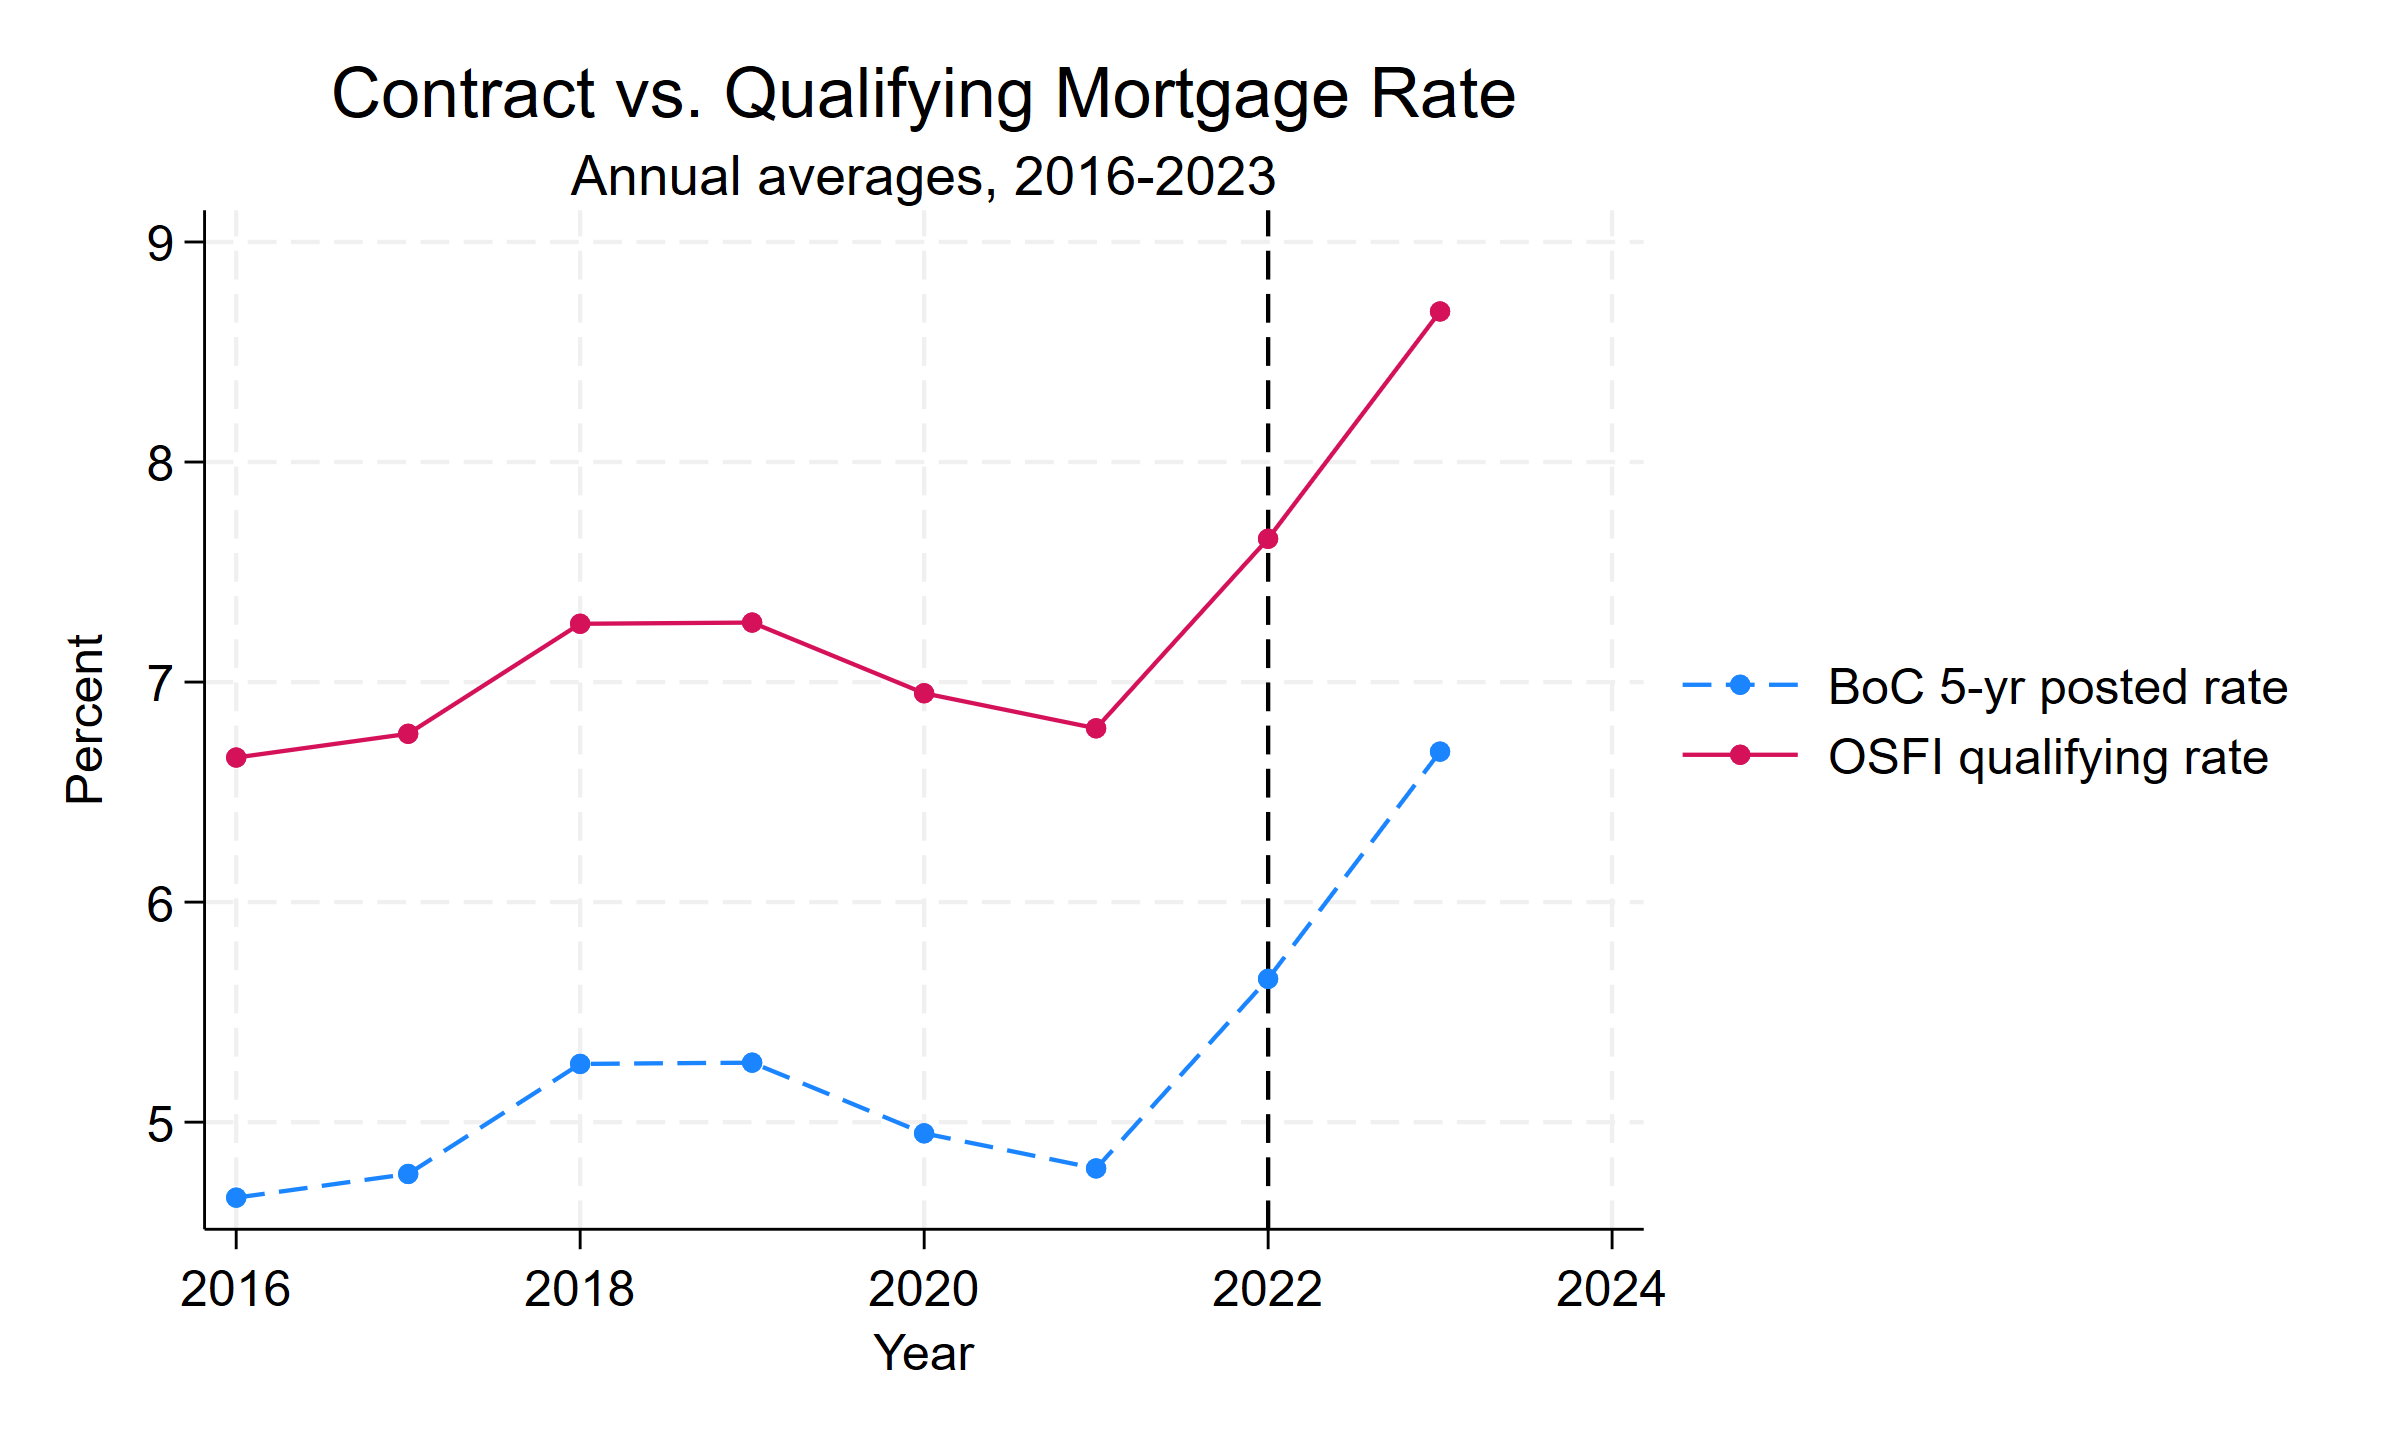
\includegraphics[width=0.74\textwidth]{qual_rate_path.png}

\caption{Contract versus qualifying mortgage rate, annual averages, 2016--2023. The qualifying rate is the greater of the contract rate plus two percentage points or the 5.25\% floor.}
\label{fig:rates}
\end{figure}

A second important consideration concerns the geographic structure of Canadian housing data. Benchmark prices are obtained from the Canadian Real Estate Association (CREA) MLS Home Price Index, which is reported by real estate boards (CREA, 2023). However, the territories of these boards do not correspond to Statistics Canada's census metropolitan areas (CMAs), which are the preferred units for analyzing urban affordability. Although most CMAs correspond to a single board, several large CMAs are covered by multiple boards, and some CMAs do not have a dedicated board. Resolving the discrepancies between these two geographic frameworks is a key data construction task, as discussed in Section~\ref{sec:proxy}.

The macroeconomic context is essential for interpreting the findings. The COVID-19 pandemic prompted an atypical relocation boom in 2020 and 2021, shifting demand from large, high-cost metropolitan areas to smaller, more affordable markets. This demand shock resulted in the largest price increases in the low-exposure markets that serve as the study's comparison group, which is crucial for understanding the subsequent results.




% =====================================================================
\section{Conceptual Framework}
% =====================================================================

A representative median-income census family in market $c$ must assess whether it qualifies to purchase the benchmark home. The maximum price that can be financed, $P^{\max}_{ct}$, decreases as the qualifying rate $r_t$ increases. An elevated qualifying rate reduces the mortgage amount a given income can support, thereby lowering the price the household can offer. The affordability gap is defined as


\begin{equation}
\text{AffordabilityGap}_{ct} \;=\; \ln P_{ct} - \ln P^{\max}_{ct},
\label{eq:gap}
\end{equation}

Here, $P_{ct}$ represents the benchmark price. A positive gap indicates that the benchmark home price exceeds the financial capacity of the median family. Conversely, a negative gap suggests that the median family can afford a home priced above the benchmark.

The effect of an increased qualifying rate on this gap is theoretically ambiguous. Interest rates influence the gap through two opposing channels, and these effects are most pronounced in high-exposure markets.

\paragraph{Capacity channel (predicts $\beta>0$).} An increase in the qualifying rate mechanically reduces $P^{\text{max}}_{ct}$. If benchmark prices remain inflexible in the short term, the resulting gap between maximum borrowing capacity and market prices widens. This effect is most pronounced in high-exposure markets, where prices substantially exceed local borrowing capacity, since an equivalent proportional reduction in borrowing capacity results in a larger absolute change in the price gap. Consequently, policy tightening amplifies the gap more significantly in higher-priced markets.

\paragraph{Price-correction channel (predicts $\beta<0$).} Higher interest rates reduce housing demand and can slow or reverse price growth. Price corrections are most significant in markets that have diverged substantially from underlying fundamentals, especially those with high exposure. As prices decline, the numerator of the valuation gap decreases, leading to the greatest narrowing in areas with the highest exposure. Therefore, the exposure interaction through this channel is negative.

Since both channels act most strongly in the same markets but in opposite directions, determining the net effect requires empirical analysis. If the capacity channel prevails, policy tightening will widen the affordability gap more in high-exposure markets ($\beta>0$, $H_1$). Conversely, if the two channels largely offset each other, or if a common national shock primarily drives the cross-market gradient, the exposure interaction will be statistically indistinguishable from zero ($\beta\approx 0$, $H_0$). The empirical results below do not reject $H_0$.


% =====================================================================
\section{Data}
\label{sec:data}
% =====================================================================

The panel dataset integrates three primary sources for the period 2016 to 2023: CREA MLS HPI benchmark prices (CREA, 2023), Statistics Canada T1 Family File (T1FF) median census-family income (Statistics Canada, 2025), and Bank of Canada five-year posted mortgage rates (Bank of Canada, n.d.), combined with the OSFI qualifying rule (OSFI, 2025). The unit of observation is the census metropolitan area (CMA) by year. The constructed panel comprises 36 CMAs observed over 8 years, resulting in 288 balanced observations, which are grouped into 35 real estate board clusters. Kelowna and Kamloops are combined within the Interior BC board, forming a single cluster. Three additional series are included solely as controls in the mechanism check in Section~\ref{sec:mechanism}, and are not part of the primary specification: CMHC housing starts by CMA (Statistics Canada, 2026c, for 2016--2020 and CMHC, 2024, for 2021--2023), population estimates by CMA (Statistics Canada, 2026b), and the annual unemployment rate by CMA (Statistics Canada, 2026a). Construction of the multi-board composite index and the proxy CMAs also draws on 2021 Census occupied-dwelling counts by board for the composite weights and on the Statistics Canada 2021 Census CMA boundary files for the geographic crosswalk described in Section~\ref{sec:proxy}. The crosswalk-construction steps and a robustness cut that reintroduces the previously dropped high-exposure markets are documented in Section~\ref{sec:proxy}.

For each market-year, the maximum qualified price $P^{\max}_{ct}$ is computed by applying a 39\% gross-debt-service allowance (CMHC, n.d.), a 25-year amortization, and a 20\% down payment (FCAC, 2025) to the median census-family income at the qualifying rate $r_t$. The affordability gap is defined according to equation~\eqref{eq:gap}. Pre-2022 exposure is calculated as each market's average price-to-income ratio over 2016--2021, standardized across markets. This measure is constructed entirely prior to the treatment period, ensuring it is not influenced by post-2022 outcomes.

The qualified price relies on two simplifying assumptions that affect only the gap level, without influencing cross-market comparisons. The 39\% allowance is attributed solely to the mortgage payment, although lenders also consider property taxes, heating, and condominium fees. This approach overstates the qualified price and understates the gap. Conversely, the posted five-year rate is higher than the discounted rates many borrowers secure, and the stress-test add-on further increases the qualifying rate. Both factors reduce the qualified price and increase the gap. Consequently, this measure should be interpreted as a conservative qualification gap, and its level is not directly comparable to the PBO's payment-affordability gap. Since both assumptions are applied uniformly across all markets and years, they are absorbed by the market and year fixed effects, leaving the estimate of $\beta$ unaffected.

Table~\ref{tab:summary} provides summary statistics. The mean benchmark price is approximately \$451,300, while the mean median census-family income is about \$95,200, resulting in a mean price-to-income ratio of 4.7. The mean log affordability gap is $-0.30$, indicating that a typical median family can qualify for slightly more than the benchmark home on average. However, there is considerable variation, with a standard deviation of 0.48 and a maximum of $+0.79$ in the most constrained market-years. The qualifying rate varies from 6.66\% to 8.68\%. Standardized exposure ranges from $-1.31$ in Trois-Rivi\`{e}res to $+3.12$ in Vancouver. Only three markets have an exposure greater than 1.5, highlighting the limited identifying variation at the upper end of the distribution.


\begin{table}[H]
\centering
\caption{Summary statistics, 36 CMAs $\times$ 8 years (2016--2023), 288 market-years.}
\label{tab:summary}

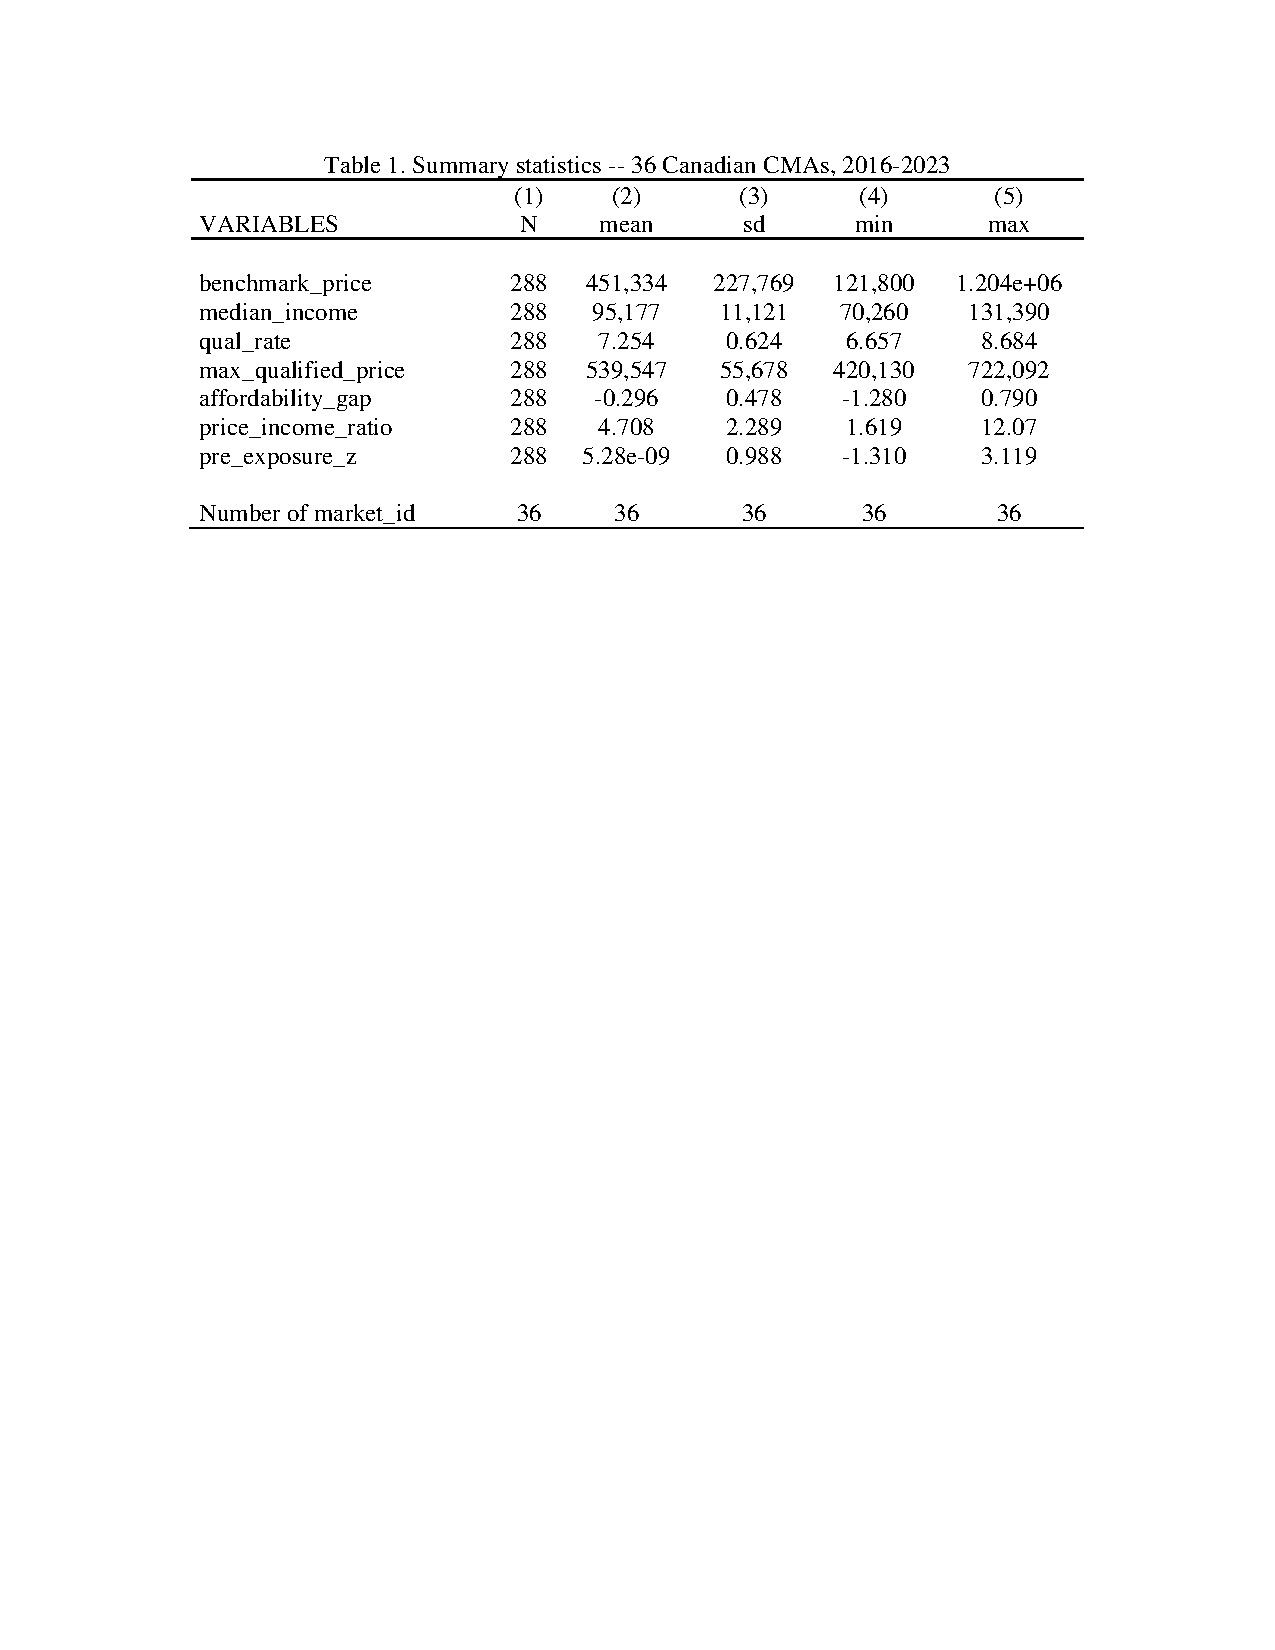
\includegraphics[width=\linewidth,height=0.5\textheight,%
        trim=0 18cm 0 1cm,clip,keepaspectratio]{tab1_summary_stats_Tran.pdf}

\smallskip
{\footnotesize \textit{Note.} Raw Stata output (\texttt{outreg2}). The row ``Number of market\_id'' confirms the balanced panel of 36 markets.}
\end{table}

\texttt{benchmark\_price} is the CREA MLS HPI composite benchmark. \texttt{median\_income} is the median before-tax income of all census families (Statistics Canada Table 11-10-0017-01). \texttt{qual\_rate} applies the OSFI rule to the Bank of Canada five-year posted rate, and \texttt{max\_qualified\_price} is the price implied by a 39\% GDS allowance, 25-year amortization, and 20\% down payment. \texttt{affordability\_gap} is $\ln(\text{price})-\ln(\text{max qualified price})$, and \texttt{pre\_exposure\_z} is the standardized 2016--2021 average price-to-income ratio. The three control series used in the mechanism check (Section~\ref{sec:mechanism}) are not shown in this table.


% ---------------------------------------------------------------------
\subsection{Constructing the CMA panel and the proxy CMAs}
\label{sec:proxy}
% ---------------------------------------------------------------------

Because CREA reports prices by real-estate board rather than by census metropolitan area (CMA), constructing a CMA-level price panel requires an explicit crosswalk. The process is organized in three tiers, and the methodological choices at this stage significantly affect both coverage and interpretation.

The crosswalk is constructed in three documented steps that are reproducible from the raw inputs. First, each CREA board is mapped to its member municipalities using CREA's published board-coverage lists, resulting in a municipality-to-board key. Second, the principal municipality of each board is geocoded and matched to the Statistics Canada 2021 Census CMA boundary files using a point-in-polygon spatial join in ArcGIS. A board point located within a CMA polygon is considered a candidate CMA match for that board. This process generates a crosswalk map in which CMA boundaries are represented as polygons and matched CREA boards as points, primarily concentrated in southern Ontario and Quebec, the Maritimes, and the BC Lower Mainland and southern interior. Third, candidate matches are confirmed or corrected by name against the CMA's principal city, and each validated match is assigned a match-quality flag (exact, GIS-confirmed, or manually anchored). The output is a single board-to-CMA correspondence file that the replication code reads directly, enabling the panel to be rebuilt from the raw CREA workbook and the boundary files without any manual intervention.

\paragraph{Tier 1: exact and near-exact matches.} 27 Census Metropolitan Areas (CMAs) correspond to a single Canadian Real Estate Association (CREA) board whose territory either matches or is centered on the CMA, including Calgary, Edmonton, Winnipeg, and Halifax. These cases do not require weighting. Combined with the 4 multi-board CMAs discussed in the following section, they constitute a 31-CMA baseline sample.

\paragraph{Tier 2: multi-board CMAs and the composite index.} 4 CMAs are served by multiple boards: Toronto (Greater Toronto, Mississauga, Oakville--Milton), Vancouver (Greater Vancouver, Fraser Valley), Kitchener--Cambridge--Waterloo (Kitchener--Waterloo, Cambridge), and Barrie (Barrie \& District, Simcoe \& District). In these cases, relying on a single-board price excludes portions of the metropolitan area. To address this, I construct a household-weighted composite House Price Index (HPI), assigning weights to each constituent board based on its proportion of the CMA's occupied private dwellings according to the 2021 Census. Since CREA does not provide board-boundary shapefiles, it is not possible to calculate the precise dwelling shares within each board's area, so the resulting weights are necessarily approximate. Consequently, the single-board series serves as the primary specification because it does not rely on unverifiable weighting assumptions, while the composite index is included solely as a robustness check using three alternative weighting schemes (Section~\ref{sec:results}).

\paragraph{Tier 3: proxy CMAs.} 5 CMAs lack dedicated boards and are instead assigned to corresponding covering boards, with match quality noted. Abbotsford--Mission is assigned to the Fraser Valley board, Nanaimo to the Vancouver Island board, Drummondville to the Centre-du-Qu\'ebec board, and both Kelowna and Kamloops to the Interior BC board. The assignment of Kelowna and Kamloops requires particular attention: although these CMAs share a single price series, they are assigned distinct income and exposure values but are grouped into one price cluster for inference to prevent double-counting of their common price shock. Including these five CMAs increases the sample to 36. Automated integrity checks confirm that the panel is strongly balanced, with each market observed for all eight years, no missing or non-positive prices, and identical Kelowna--Kamloops price series.

\paragraph{Reintroducing the dropped markets, and what cannot be recovered.} The markets excluded from the earlier 31-CMA build were disproportionately high-exposure British Columbia markets, resulting in selection bias on the variable whose interaction is estimated. The Tier-3 expansion directly addresses this issue by reintroducing five of these markets (Abbotsford--Mission, Nanaimo, Kelowna, Kamloops, and Drummondville; four are high-exposure BC markets) through proxy-board matching with flagged match quality. As a result, the 36-CMA sample is no longer selected based on exposure. Of Canada's 41 Census Metropolitan Areas (CMAs) according to the 2021 Census, five remain outside the sample: Oshawa, Saguenay, Lethbridge, Thunder Bay, and Red Deer. Four of these lack overlapping CREA board series in the source workbook, making it impossible to construct a price index for them without fabricating data. Oshawa is an instructive exception, as its territory is included within the Toronto board's aggregate, preventing separation without double-counting the same price series. These five CMAs are therefore omitted transparently rather than proxied. The final sample includes 36 of 41 CMAs (88\%) and employs a single, consistent unit of analysis throughout.



% =====================================================================
\section{Methods}
\label{sec:methods}
% =====================================================================

The main specification is a continuous-treatment difference-in-differences model estimated by two-way fixed effects:
\begin{equation}
\text{AffordabilityGap}_{ct} \;=\; \alpha_c \;+\; \lambda_t \;+\; \beta\,\big(\text{QualRate}_t \times \text{PreExposure}_c\big) \;+\; \varepsilon_{ct},
\label{eq:main}
\end{equation}
where $c$ indexes the 36 markets and $t$ indexes years 2016--2023. Market fixed effects $\alpha_c$ account for permanent differences across markets, including the time-invariant level of pre-exposure. Year fixed effects $\lambda_t$ account for the national qualifying rate $\text{QualRate}_t$ and any other shocks common to all markets within a given year. Because $\text{QualRate}_t$ varies only over time and $\text{PreExposure}_c$ varies only across markets, each is absorbed by a distinct set of fixed effects. Identification therefore relies exclusively on their interaction, which varies at the market-year level. Standard errors are clustered at the real-estate-board level, corresponding to the level at which the price treatment is assigned. The coefficient $\beta$ represents the additional log-point change in the gap per one-percentage-point increase in the qualifying rate, for a market one standard deviation above the mean exposure. The primary specification does not include time-varying controls; supply and demand controls are introduced separately as an exploratory mechanism check in Section~\ref{sec:mechanism}.


\paragraph{Causal or correlational?} I interpret $\beta$ as a correlational parameter rather than a causal one. Pre-2022 exposure is not randomly assigned. Instead, it reflects decades of local supply constraints, income growth, and location-specific demand. The two-way fixed-effects structure accounts for time-invariant market differences and common time shocks. However, it does not eliminate the influence of time-varying, market-specific factors correlated with both exposure and the gap, with the pandemic relocation boom serving as a primary example. Callaway et al. (2024) demonstrate that a continuous-treatment design of this nature identifies a causal parameter only if a parallel-trends condition holds across the entire support of the treatment. I test this condition directly below and, in the extension, find that it fails once the common shock is absorbed at the regional level.


\paragraph{The mean-reversion caveat.} The primary threat to interpretation is mechanical mean reversion. Pre-exposure is defined as the average price-to-income ratio from 2016 to 2021. Once the qualifying rate is standardized across all markets within a given year, the affordability gap closely tracks the current price-to-income ratio. Consequently, when year fixed effects absorb the national rate, the interaction effectively compares each market's current price-to-income ratio to its historical level. This process tends to generate a negative coefficient by construction, irrespective of whether policy tightening elicited any behavioral response. This dynamic provides a plausible alternative explanation for the small negative estimate, supporting the interpretation of the result as correlational rather than causal. It remains challenging to distinguish a genuine price-correction effect from markets merely reverting toward their previous price-to-income levels. This issue is revisited in the interpretation of the results and represents the most significant caveat to the paper's findings.

\paragraph{Inference with few clusters.} With 35 clusters, conventional cluster-robust $t$-based $p$-values can over-reject (Cameron et al., 2008; MacKinnon \& Webb, 2018). I therefore complement the asymptotic inference with a wild cluster bootstrap (Rademacher weights, 9{,}999 replications, null imposed) via \texttt{boottest} (Roodman et al., 2019).


% =====================================================================
\section{Results}
\label{sec:results}
% =====================================================================

Table~\ref{tab:main} reports the primary estimates and results from the leave-out robustness analysis. In the main specification, column~(1), the exposure interaction coefficient is $\hat{\beta}=-0.0145$ with a cluster-robust standard error of $0.0128$ ($p=0.264$). In level terms, a one-standard-deviation increase in pre-2022 exposure is associated with a 1.45\% smaller increase in the affordability gap for each one-percentage-point rise in the qualifying rate. The qualifying rate increased by approximately two percentage points between 2021 and 2023, implying an estimated 3\% differential between high- and average-exposure markets. This effect is economically modest. The 95\% confidence interval ($-0.041$ to $+0.011$) contains zero as well as both small positive and negative values. The point estimate is opposite in sign to the capacity-channel prediction ($H_1$). However, its lack of statistical significance suggests that the data do not support either a positive or negative gradient. The wild cluster bootstrap $p$-value is $0.39$, which exceeds the asymptotic value, as is typical when a small number of clusters leads the asymptotic test to over-reject. Therefore, the null hypothesis appears even more robust under conservative inference.


\begin{table}[H]
\centering
\caption{Continuous-treatment difference-in-differences estimates.}
\label{tab:main}

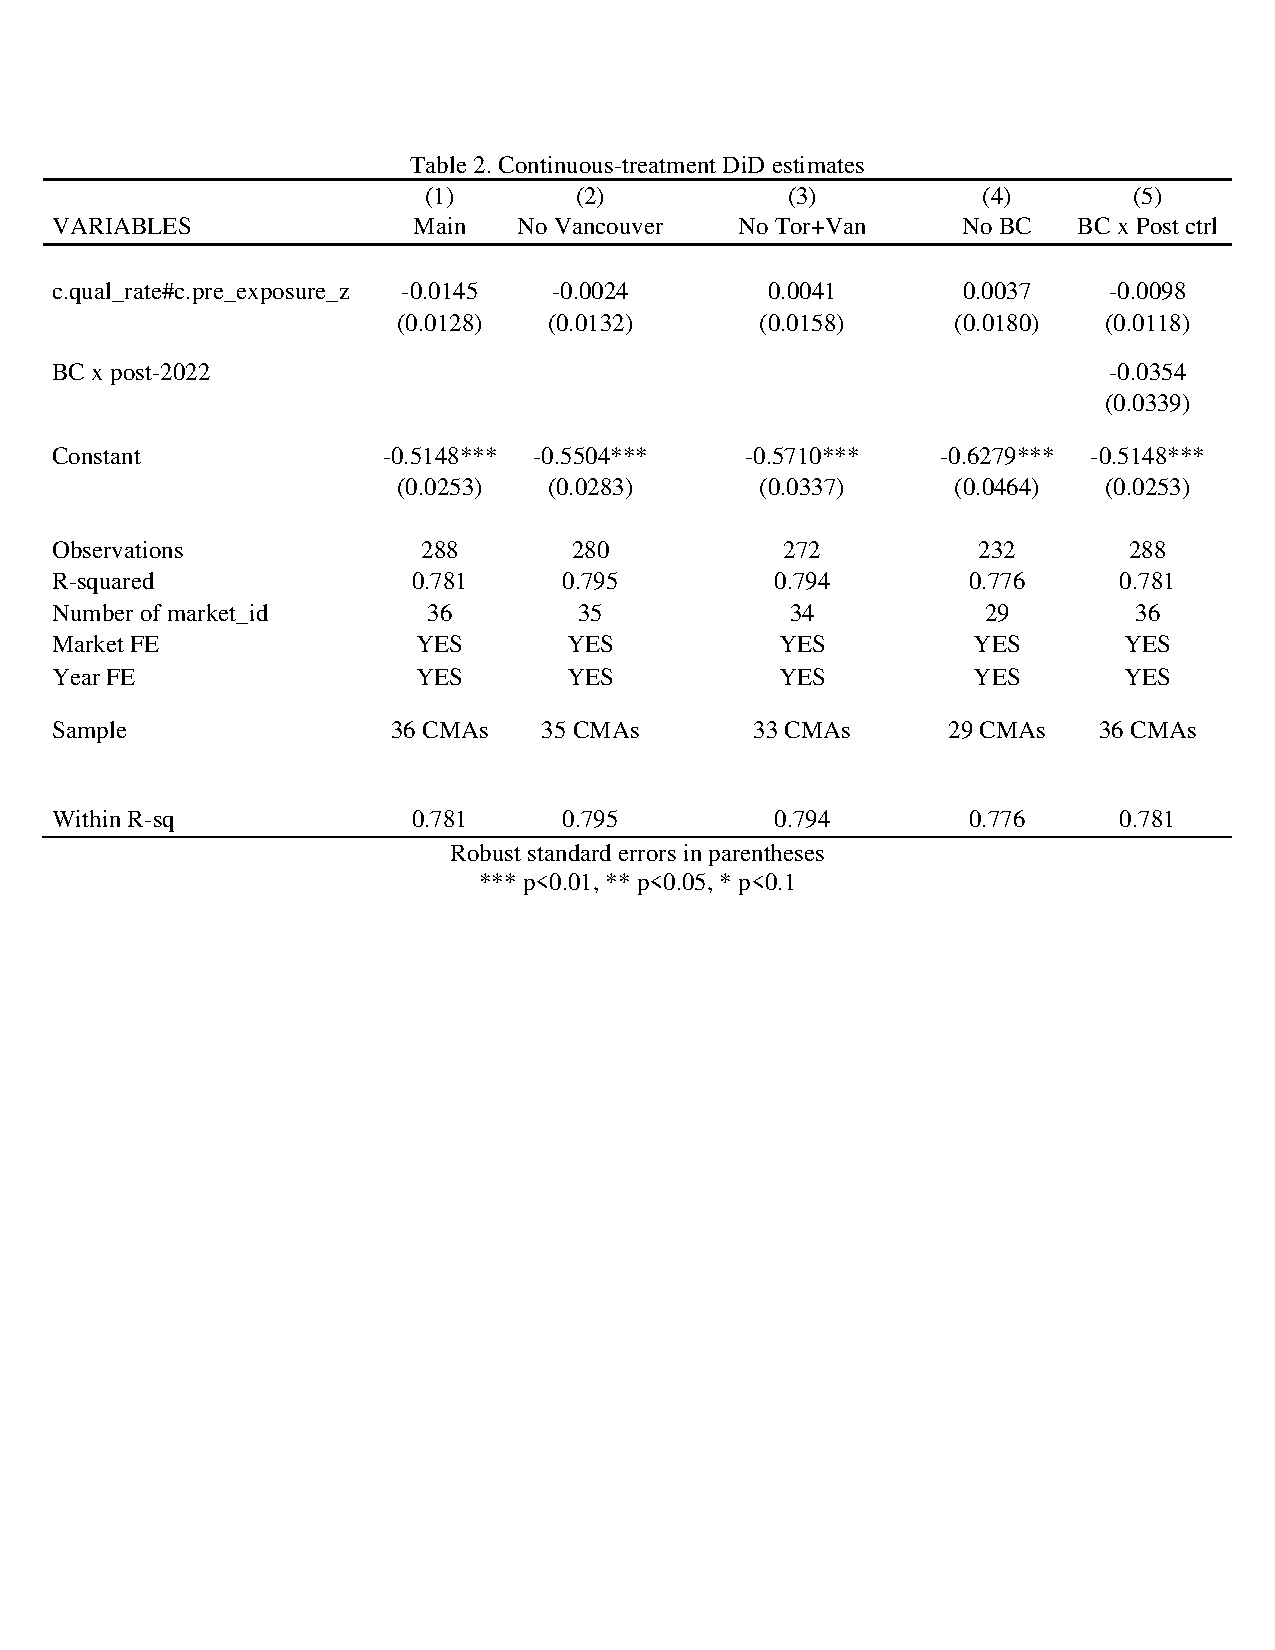
\includegraphics[width=\linewidth,height=0.5\textheight,%
        trim=0 12cm 0 1cm,clip,keepaspectratio]{tab2_main_results_Tran.pdf}

\smallskip
{\footnotesize \textit{Note.} Raw Stata output (\texttt{outreg2}). All columns include market and year fixed effects; cluster-robust standard errors (by CREA board) in parentheses.}
\end{table}

The dependent variable is the affordability gap. Column~(1) is the primary 36-CMA specification. Columns~(2) to (4) drop Vancouver, Toronto and Vancouver, and all British Columbia markets respectively, and column~(5) adds a British Columbia $\times$ post-2022 indicator. No exposure-interaction coefficient is significant at the 10\% level, and the wild cluster bootstrap $p$-value for column~(1) is $0.39$.

\paragraph{The gradient is a two-market artifact.} The decisive pattern appears in columns (2)--(4). Excluding Vancouver alone shifts the estimate from $-0.0145$ to $-0.0024$; excluding both Toronto and Vancouver moves it to $+0.0041$; and excluding all of British Columbia leaves it at $+0.0037$. In each case the estimate is statistically indistinguishable from zero and, if anything, weakly positive. A formal leave-one-market-out diagnostic confirms the source: re-estimating $\hat{\beta}$ 36 times, each time dropping one market, Vancouver's standardized influence on the estimate is 4.6 times that of the typical market, by far the largest in the sample (reported in the replication log rather than Table~\ref{tab:main}). The year effects absorb the common shock, but they do not neutralize the leverage a single outlier exerts on a cross-sectional slope. The entire negative gradient is thus generated by two structurally atypical mega-markets and the wider BC market, which are subject to province-specific forces---foreign-buyer and speculation taxes and the federal foreign-buyer ban---that the design cannot isolate. Adding a BC $\times$ post-2022 control that nets out a BC-specific level shift with a single parameter (column 5) leaves the estimate small and insignificant ($-0.0098$, $p=0.41$).

\paragraph{Why the effect is small: a dominant common shock.} Figure~\ref{fig:terciles}a presents the mean affordability gap over time by pre-2022 exposure tercile. The three groups occupy distinct levels, with the high-exposure group exhibiting a persistently higher gap. However, the trajectories of all groups are largely parallel, and each group experiences a simultaneous increase after 2021 as tightening measures take effect. The estimated year effects indicate a common post-2021 increase of approximately half a log point (the 2022 and 2023 year coefficients are about $+0.49$), which outweighs any divergence in slopes across terciles. This pattern visually corresponds to the small $\hat{\beta}$, suggesting that tightening compressed affordability by a similar magnitude across all groups, thereby limiting the explanatory power of exposure differentials. Figure~\ref{fig:terciles}b, which re-centres each market on its 2021 value, reinforces this observation and further demonstrates that the low-exposure group's gap increases slightly more after 2022. This provides an early, model-free indication that the differential effect may run counter to the capacity-channel hypothesis.



\begin{figure}[H]
\centering
\begin{minipage}{0.49\textwidth}\centering
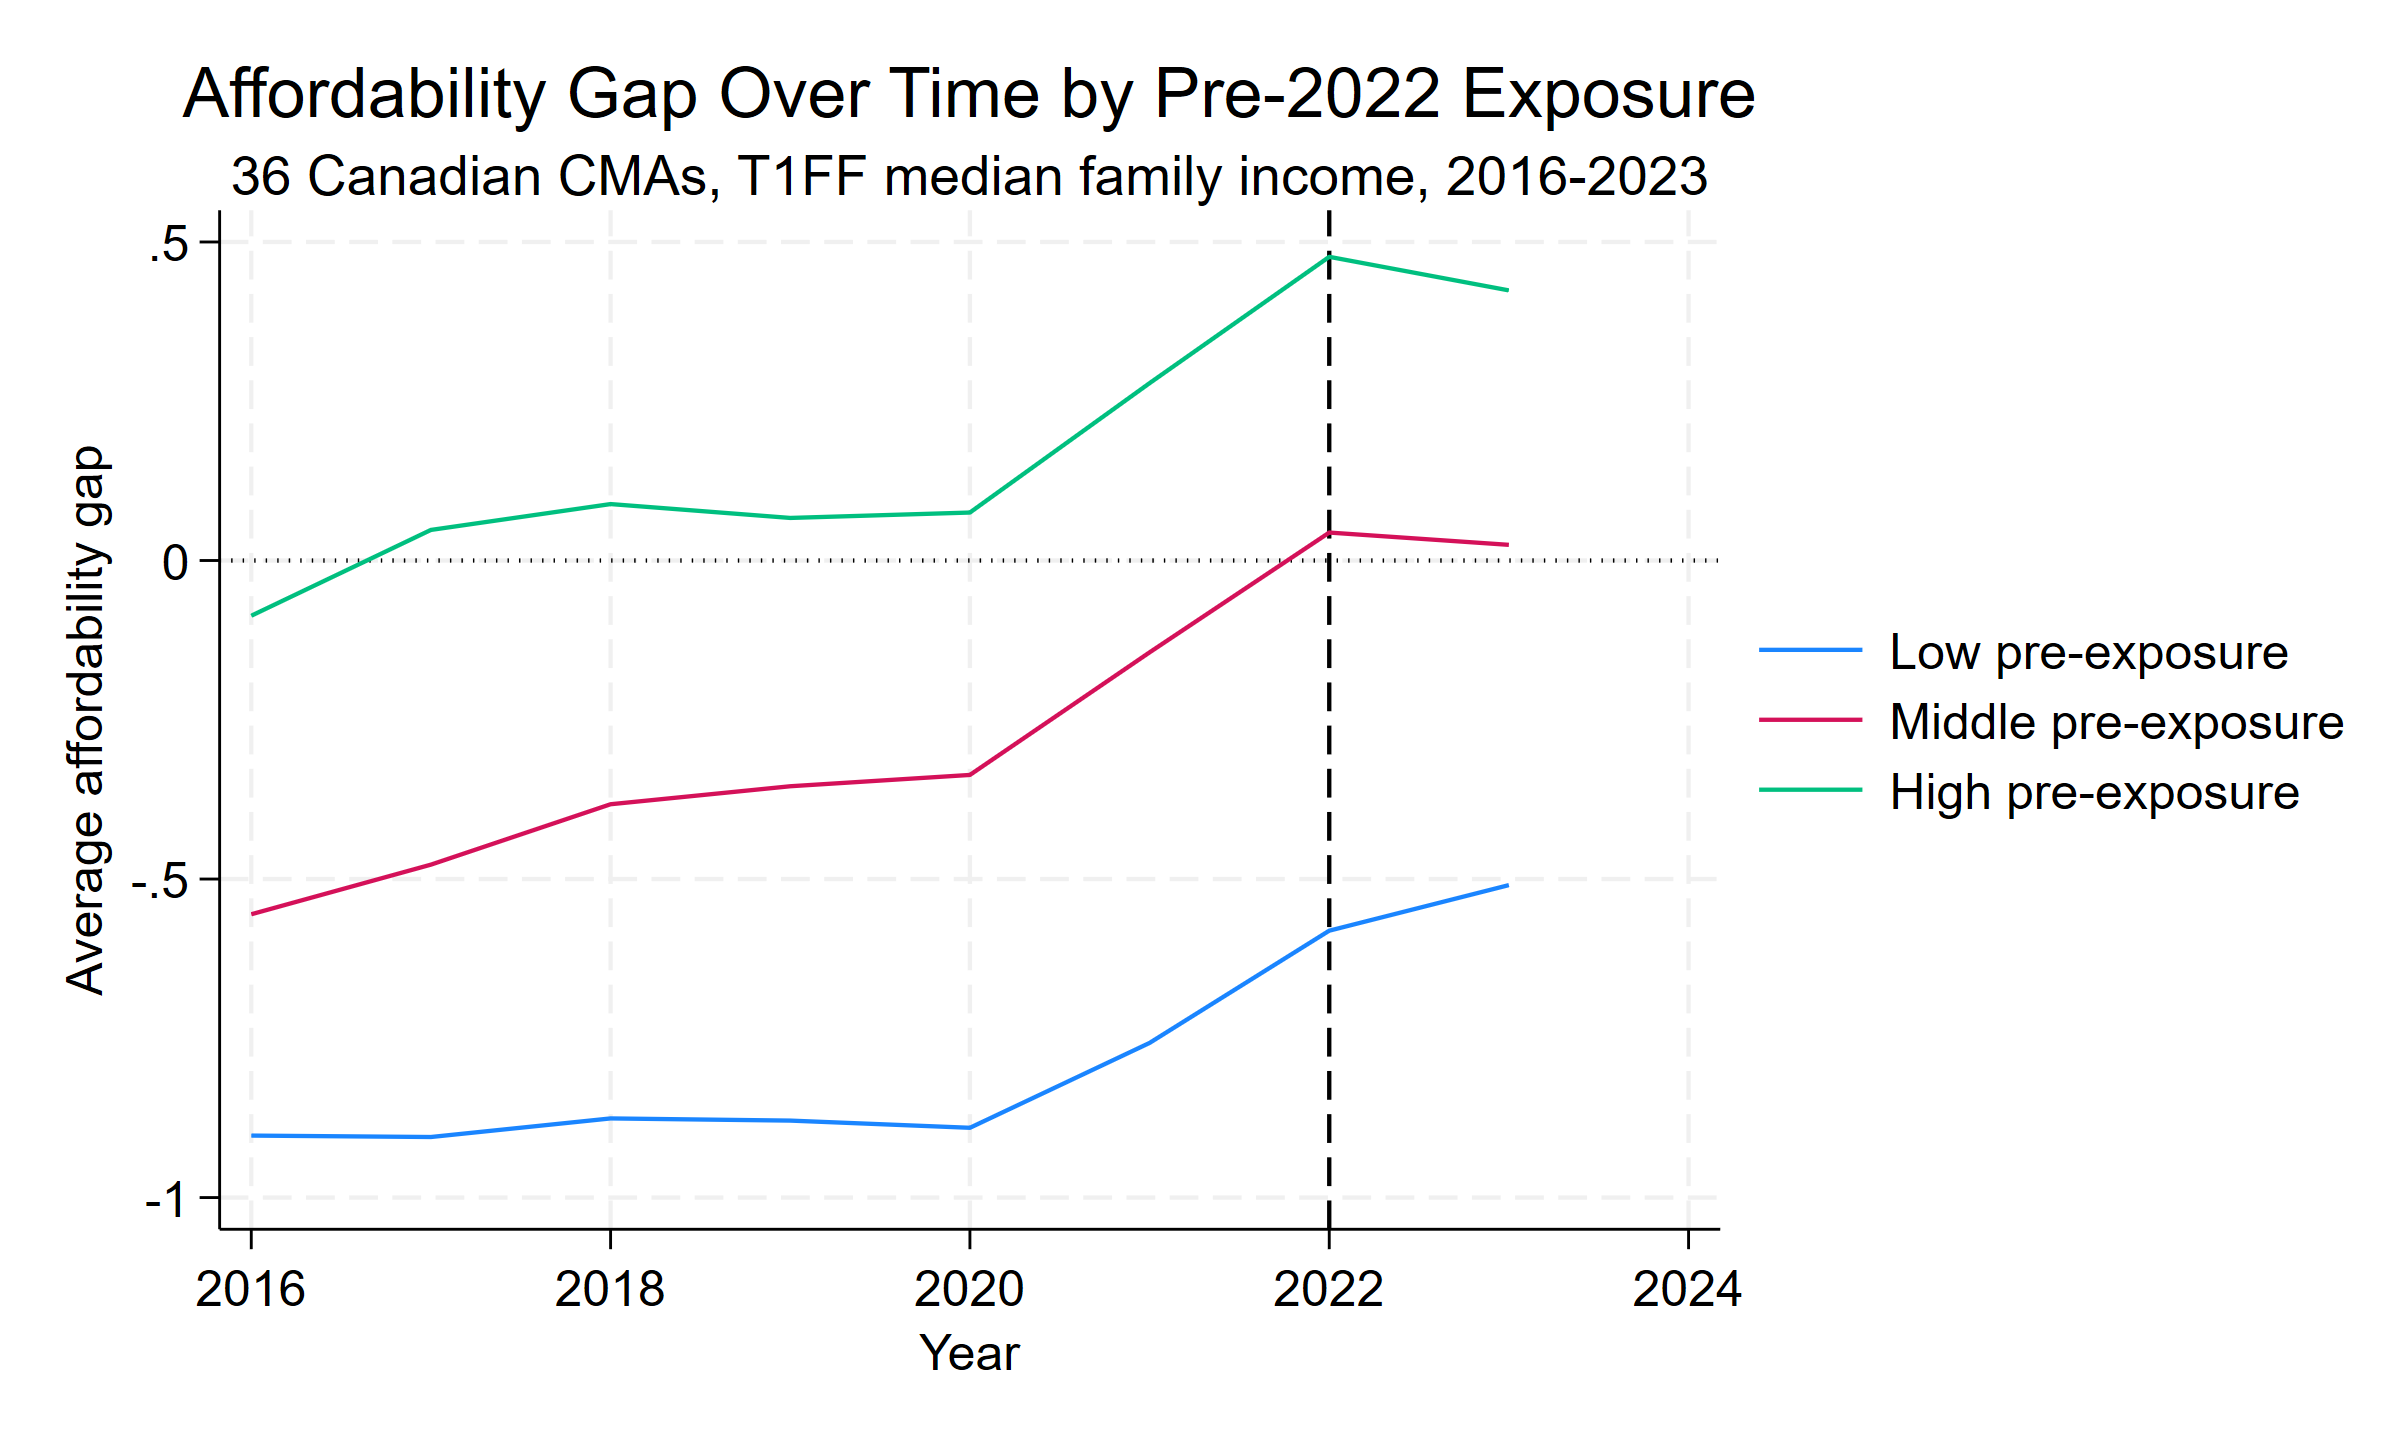
\includegraphics[width=\textwidth]{fig1_gap_by_exposure_tercile_Tran.png}\\
{\footnotesize (a) Levels}
\end{minipage}\hfill
\begin{minipage}{0.49\textwidth}\centering
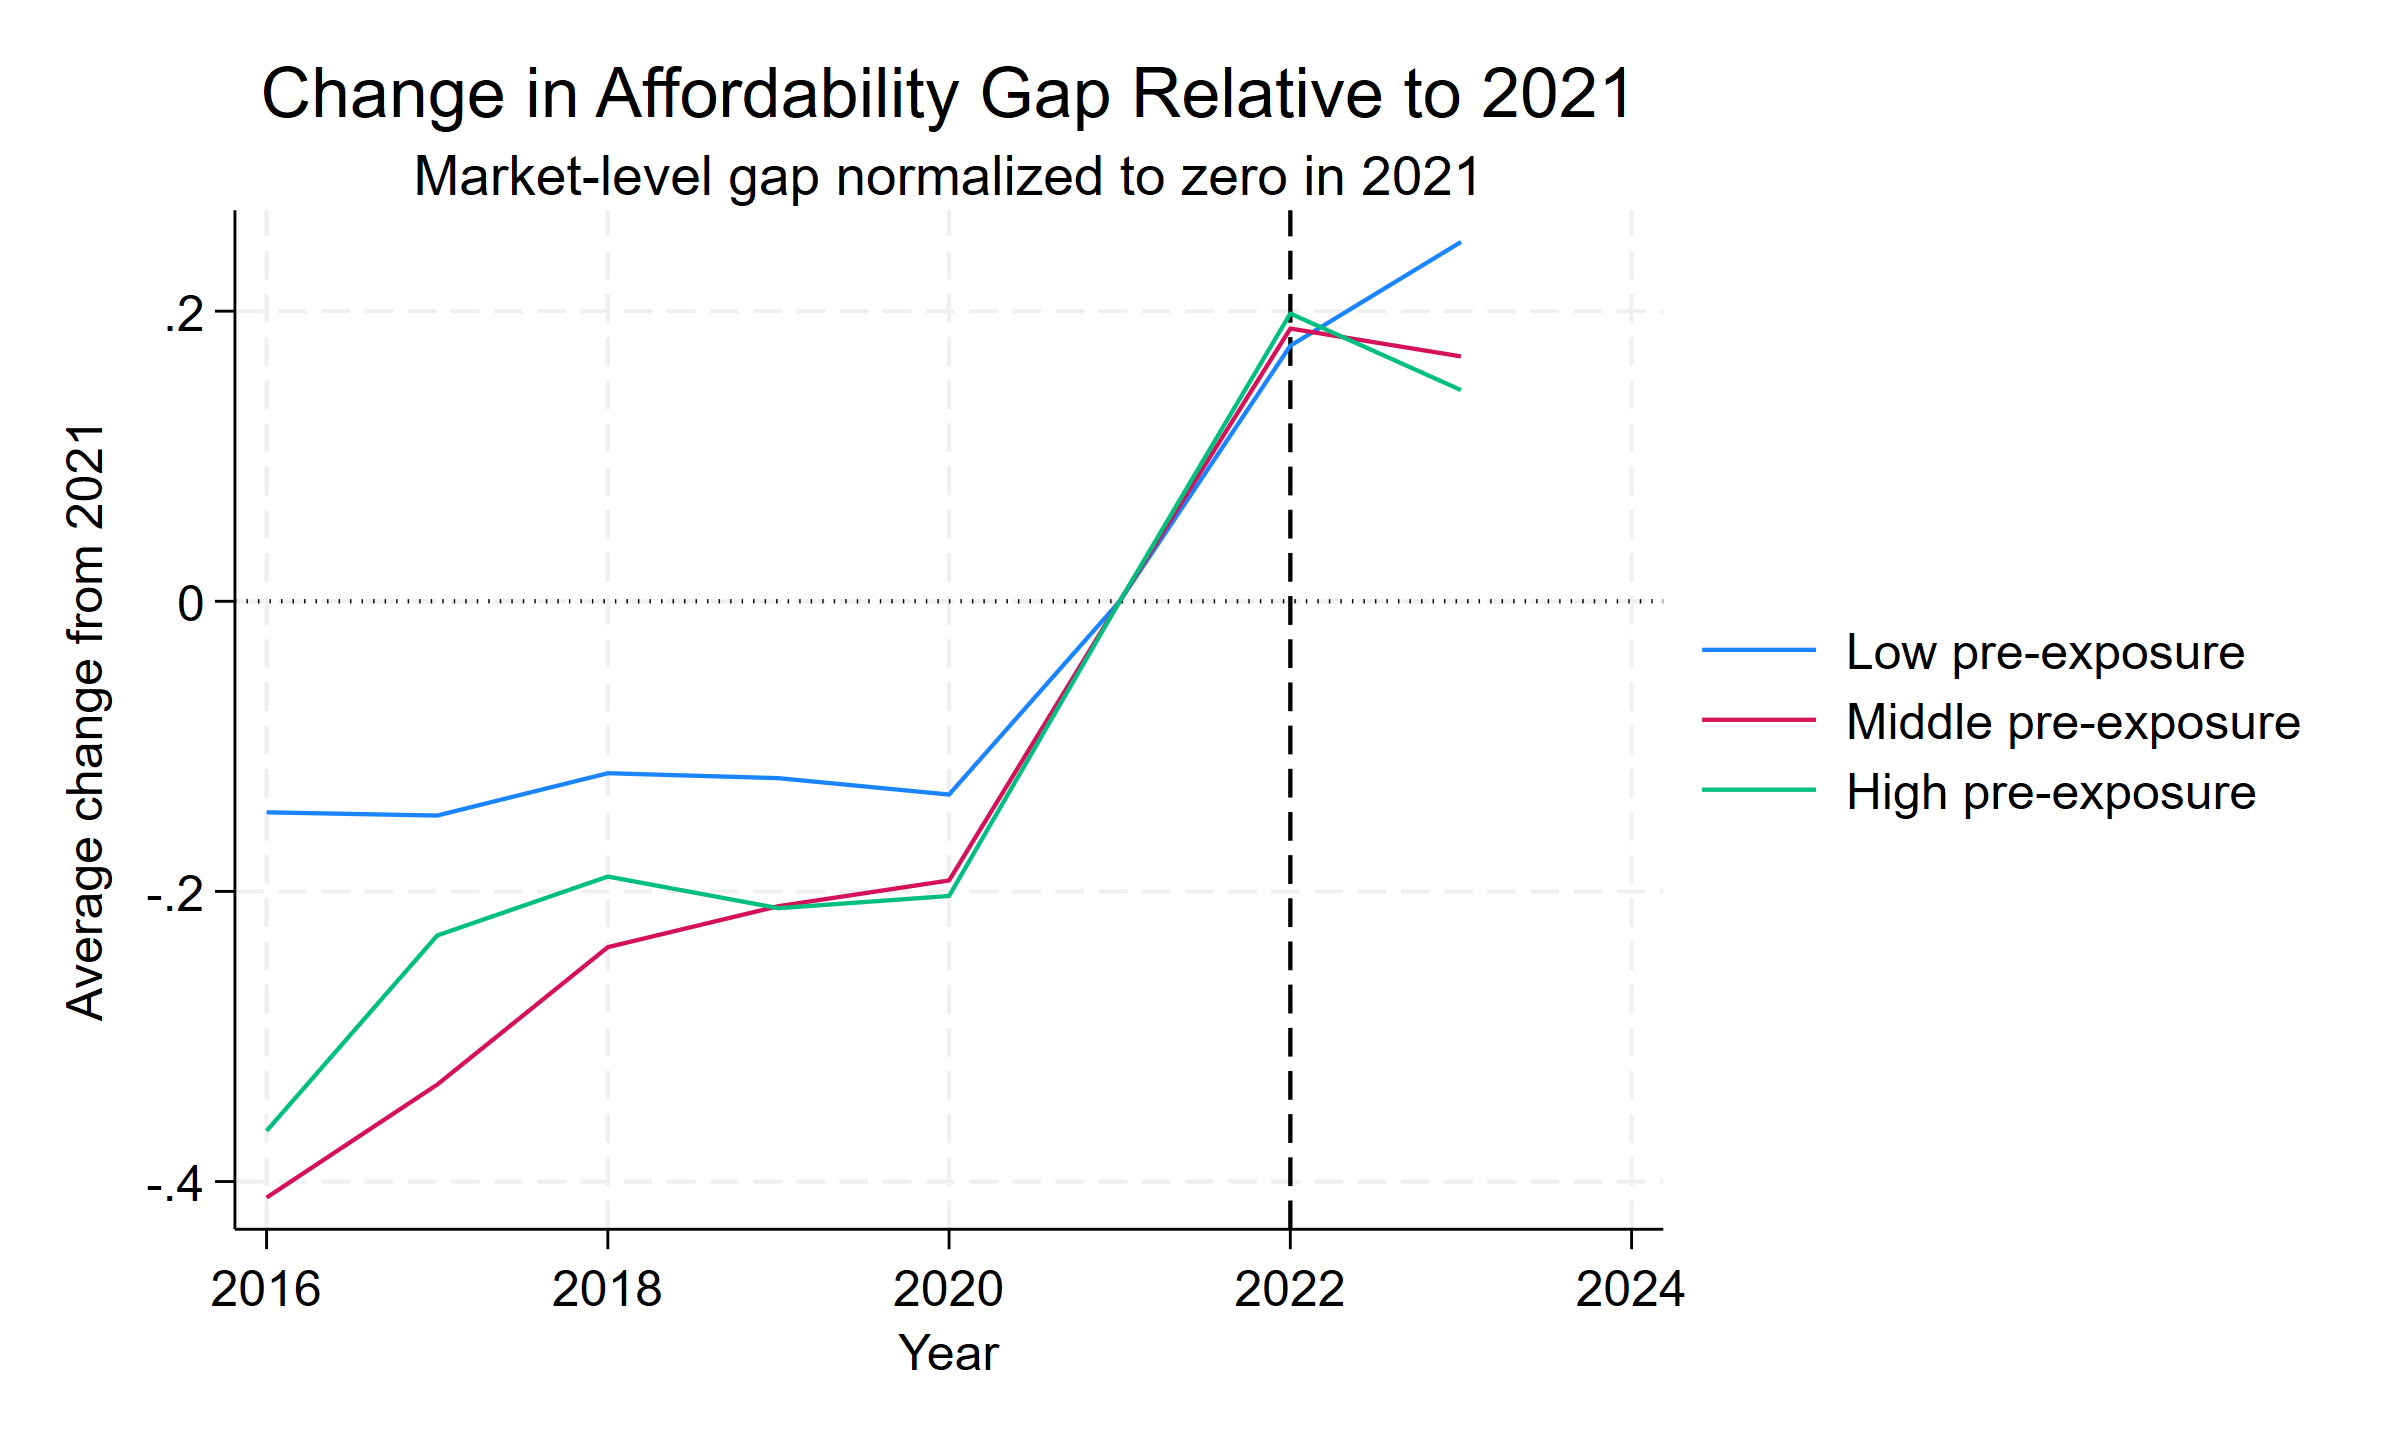
\includegraphics[width=\textwidth]{fig2_gap_relative_2021_by_tercile_Tran.png}\\
{\footnotesize (b) Relative to 2021}
\end{minipage}
\caption{Average affordability gap over time by pre-2022 exposure tercile, 36 CMAs. All three terciles rise together after the 2022 tightening, indicating a dominant common shock.}
\label{fig:terciles}
\end{figure}

\paragraph{The raw cross-section slopes the ``wrong'' way and why that is expected.} Figure~\ref{fig:scatter} presents the raw change in the affordability gap from 2021 to 2023 against pre-2022 exposure. The fitted line slopes downward: the most affordable markets (Trois-Rivi\`{e}res, Moncton, Drummondville) experienced the largest deterioration, while the most exposed markets (Toronto, Vancouver) experienced among the smallest changes. At first glance, this pattern appears to contradict the capacity channel. However, this is the raw, uncontrolled relationship, which is largely influenced by the pandemic relocation boom that drove the sharpest price increases in the low-exposure markets. The fixed-effects model in equation~\eqref{eq:main} is designed to account for this common, time-varying shock. The near-zero controlled estimate is consistent with the downward raw slope once the relocation surge in affordable markets is absorbed by the year fixed effects. This pattern is also consistent with mechanical mean-reversion, which is why the controlled estimate should not be interpreted as evidence of a behavioural price-correction effect.


\begin{figure}[H]
\centering
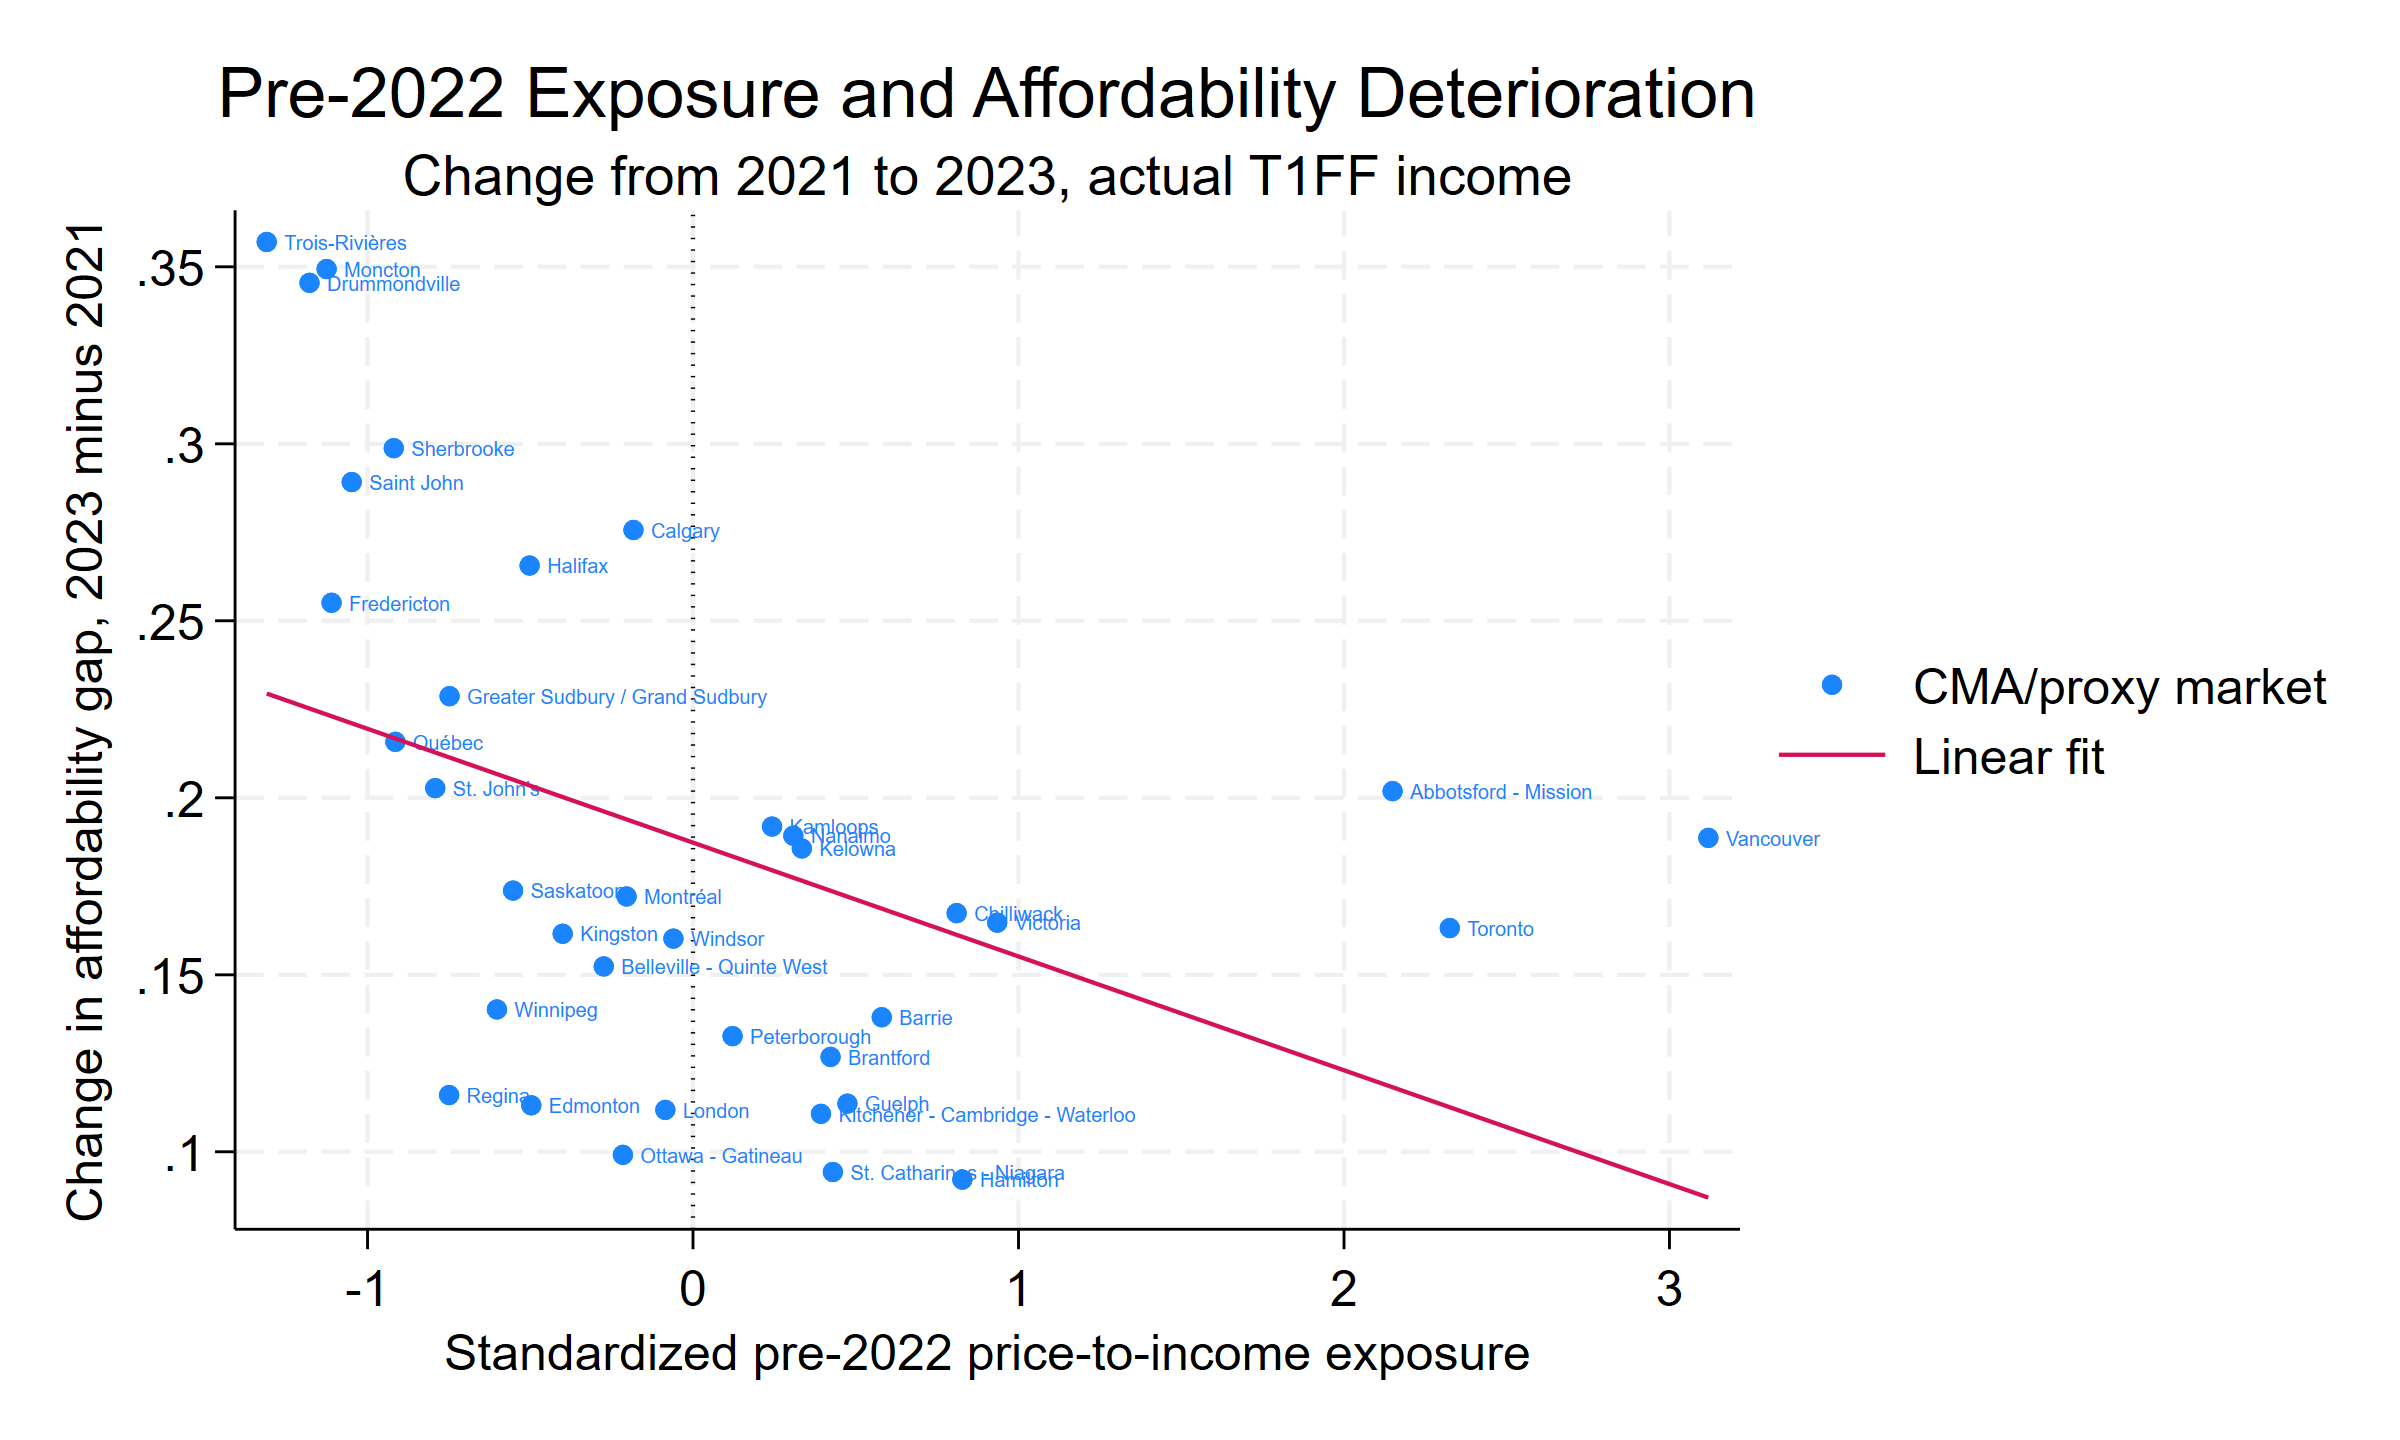
\includegraphics[width=0.72\textwidth]{fig3_exposure_vs_gap_change_2021_2023_Tran.png}
\caption{Uncontrolled change in the affordability gap, 2021--2023, against pre-2022 exposure.}
\label{fig:scatter}
\end{figure}

\paragraph{Parallel pre-trends.} Figure~\ref{fig:event} presents an event-study version of the model, displaying the exposure gradient for each year relative to 2021. The pre-2022 coefficients are small, individually insignificant, and close to zero (each $|t|<0.55$, with $p$-values between 0.59 and 0.75), which supports the parallel-trends assumption underlying the design. Although a joint Wald test of the five pre-period interactions rejects the null, this result is a mechanical artifact of near-collinear pre-period estimates with very tight standard errors. The event-study figure and the individual coefficients, rather than the over-powered joint test, provide the primary evidence for the parallel-trends assumption.


\begin{figure}[H]
\centering
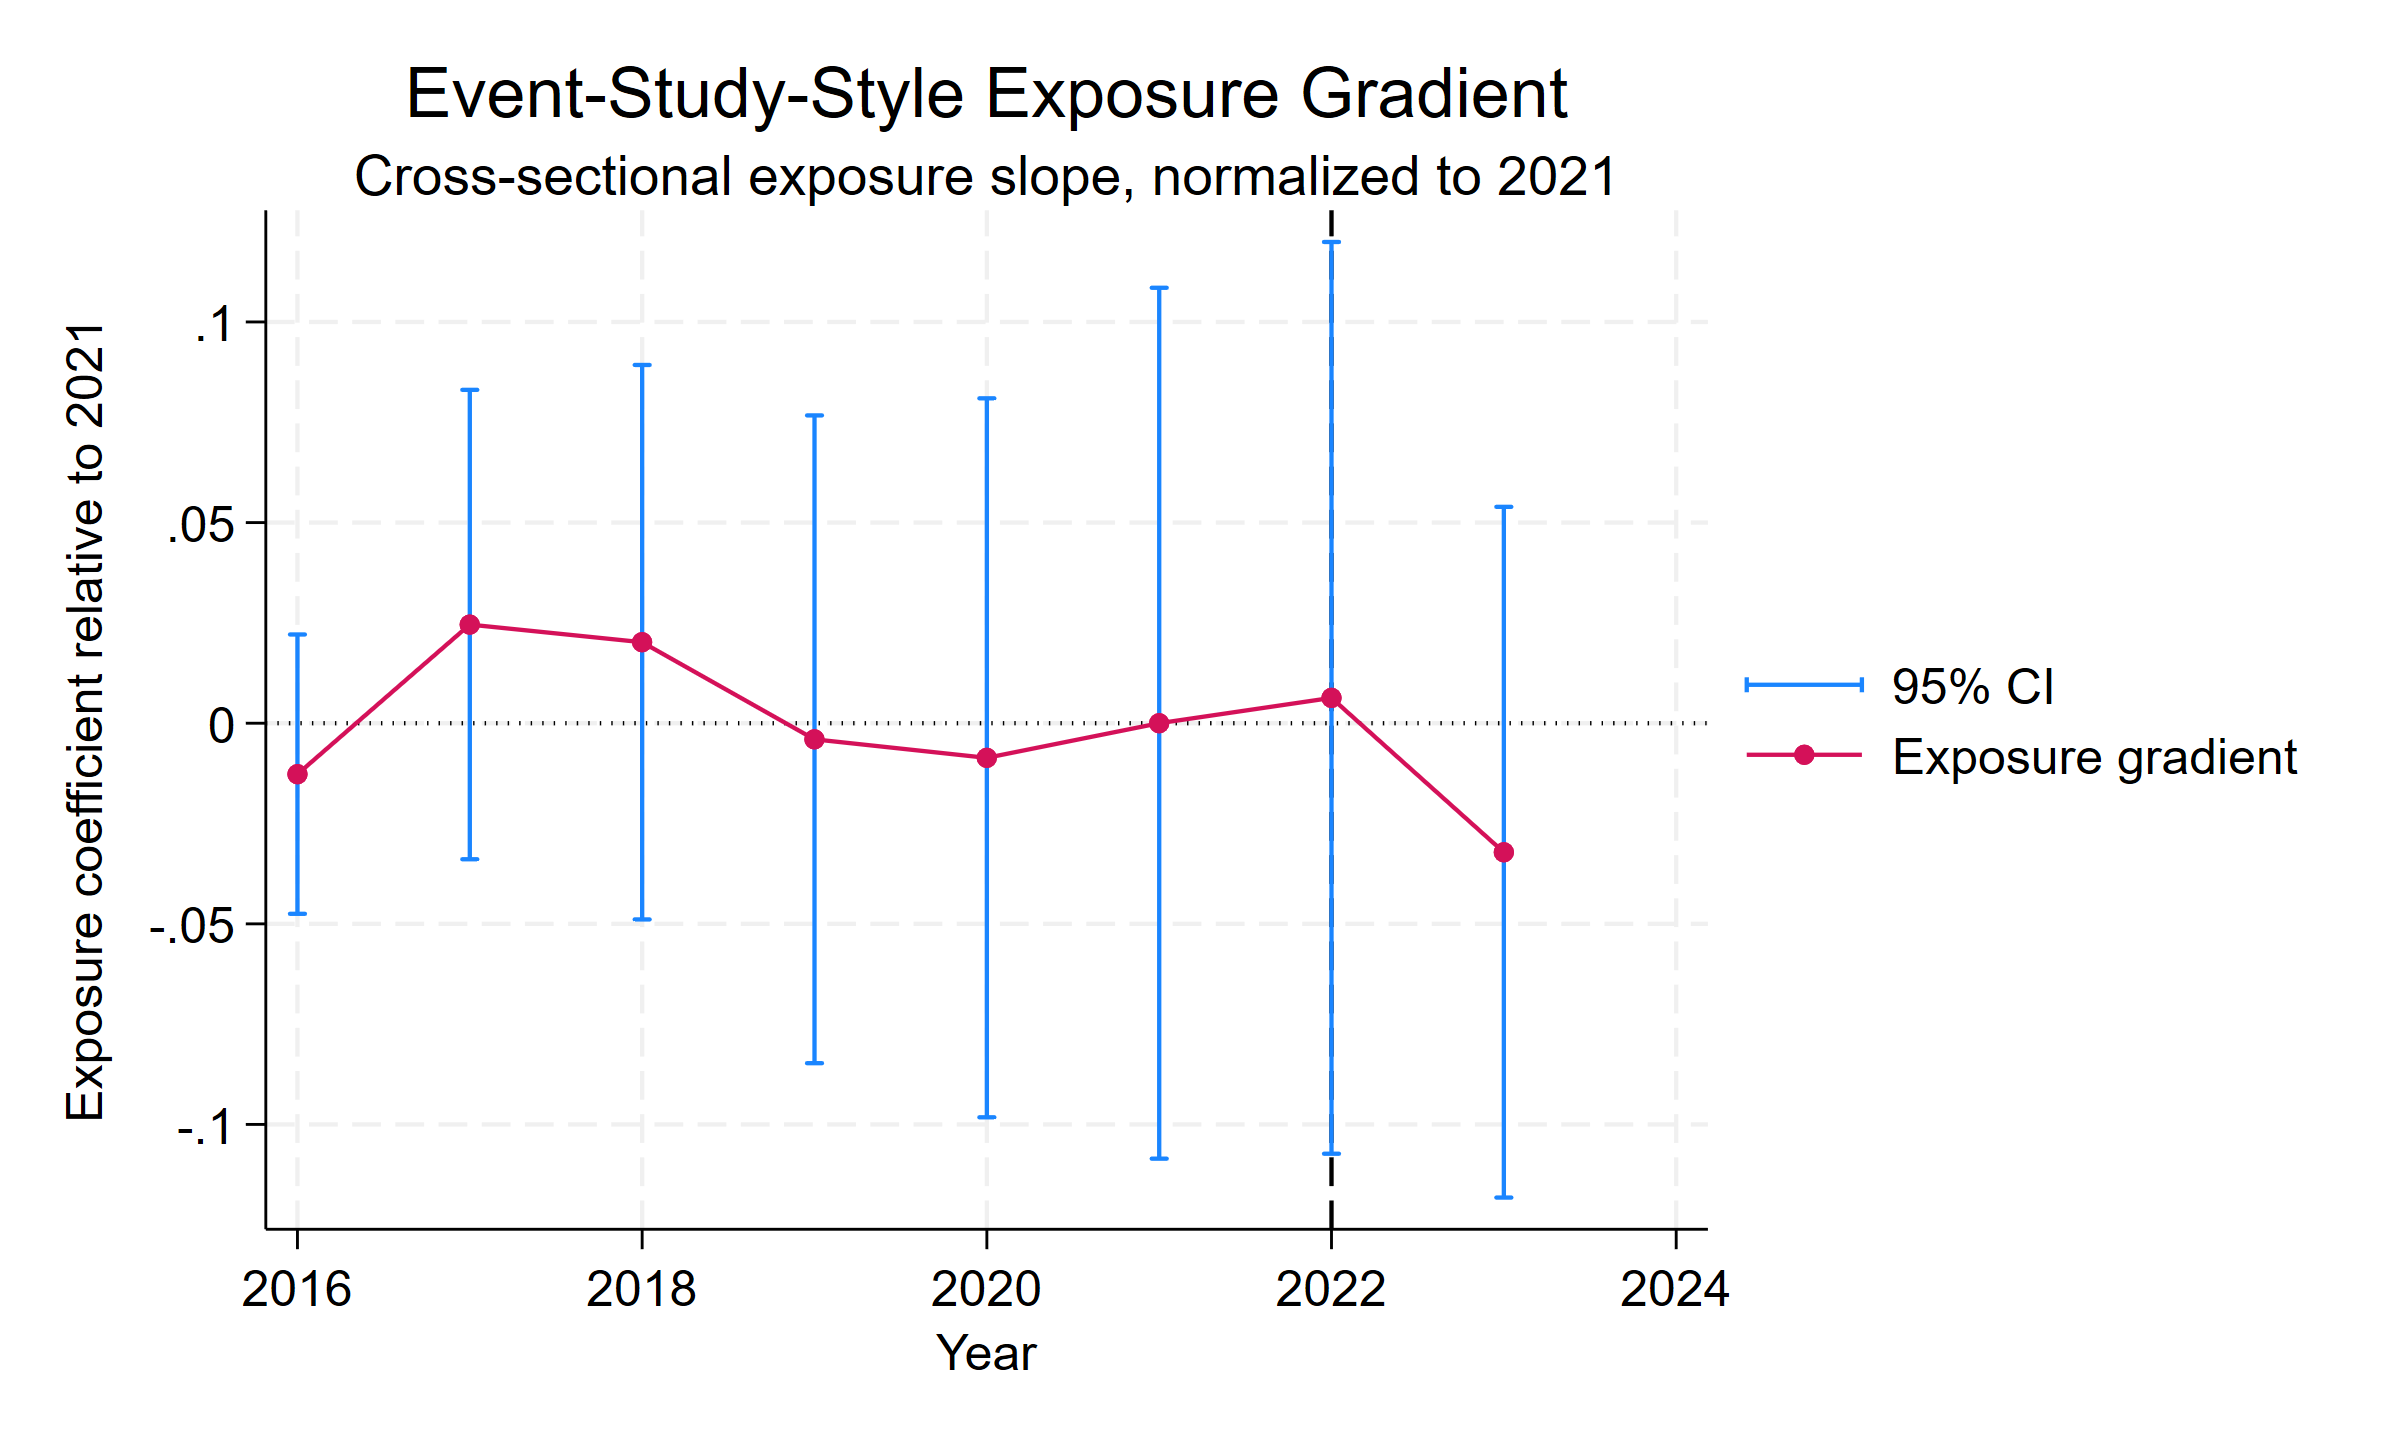
\includegraphics[width=0.72\textwidth]{fig4_event_style_exposure_gradient_Tran.png}
\caption{Event-study exposure gradient with 95\% confidence intervals, normalized to 2021. Pre-2022 coefficients are flat and individually insignificant, consistent with parallel trends.}
\label{fig:event}
\end{figure}

\paragraph{Robustness to house-price construction.} Table~\ref{tab:composite} presents re-estimates of the primary specification using the household-weighted composite HPI for the four multi-board CMAs under three weighting schemes: approximate dwelling-share, equal-weight, and population-share. The estimates remain stable across all schemes ($-0.0102$ to $-0.0145$, all statistically insignificant), indicating that the use of approximate weighting due to the absence of CREA boundary files does not influence the results. This finding directly addresses concerns that the multi-board CMAs, including the two largest markets, may be sensitive to the method used to combine their constituent boards.


\begin{table}[H]
\centering
\caption{Robustness to house-price index construction.}
\label{tab:composite}

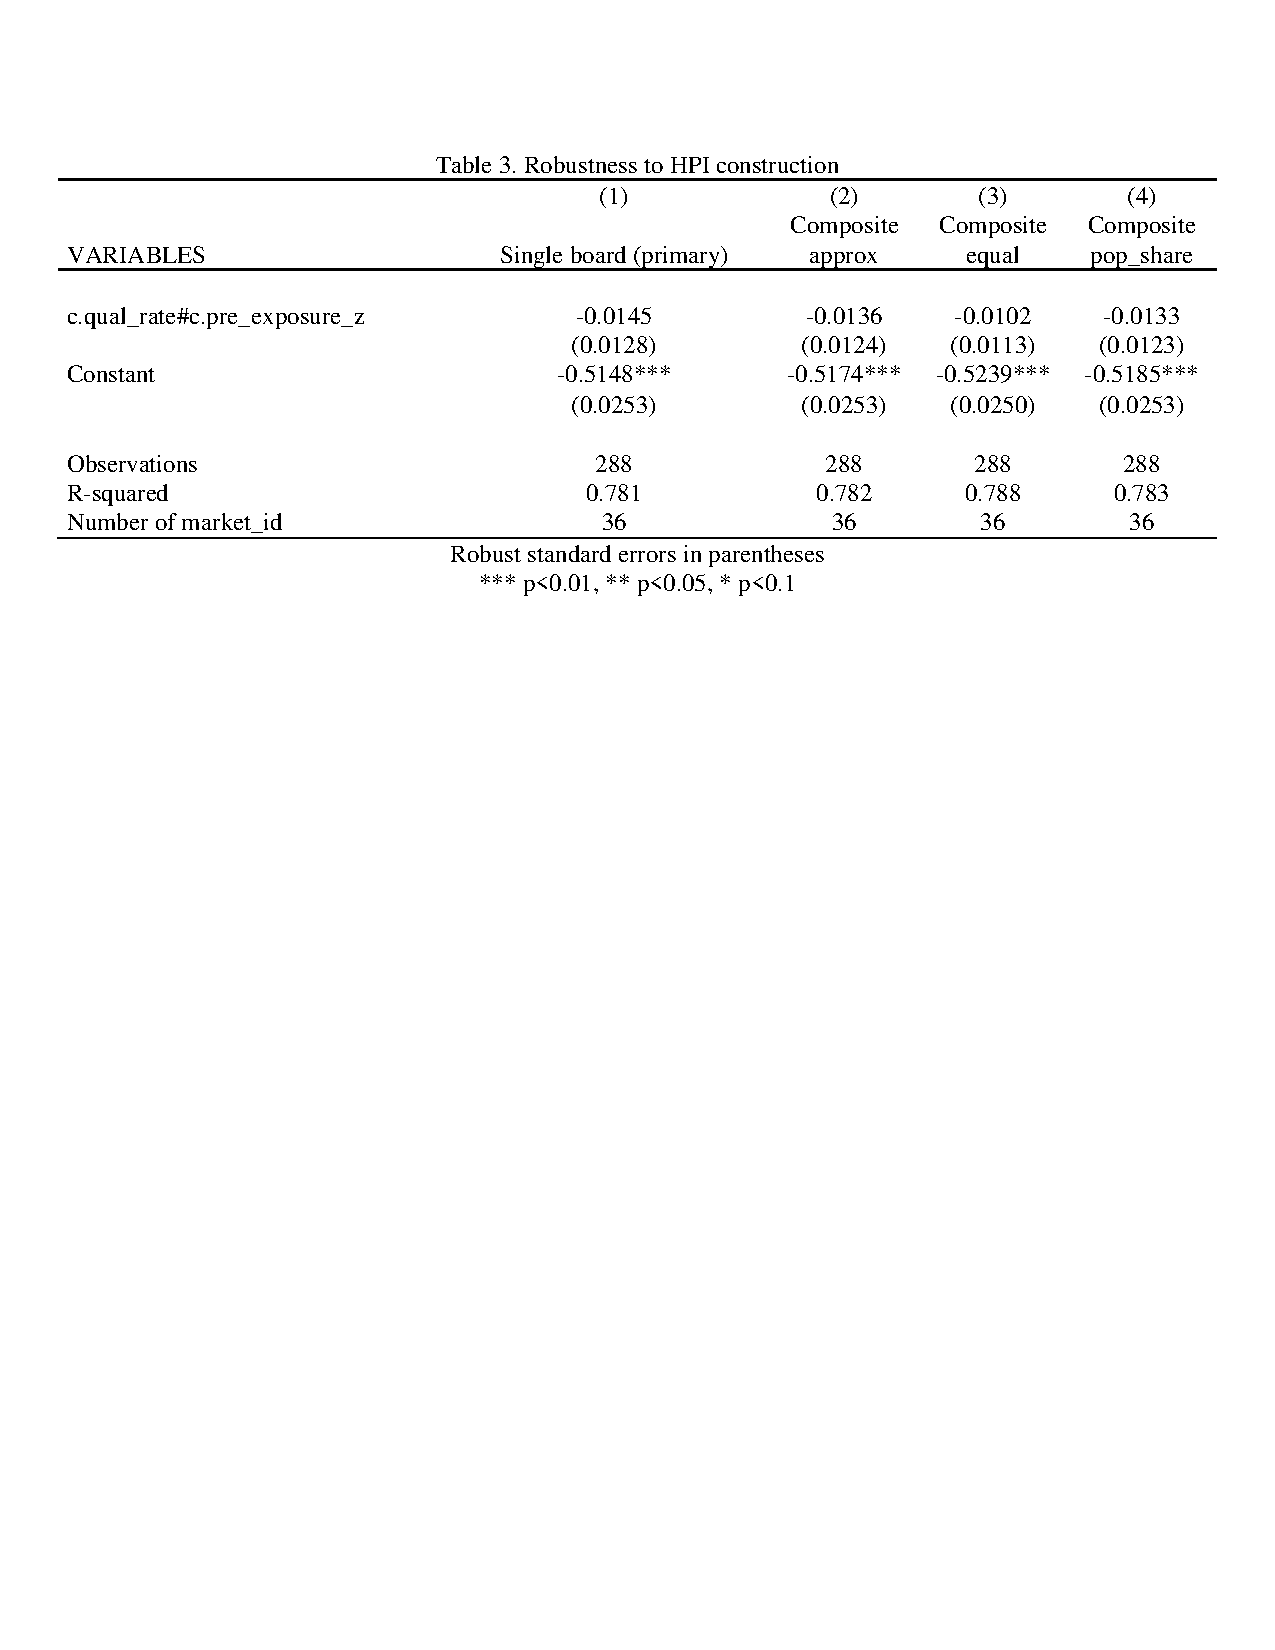
\includegraphics[width=\linewidth,height=0.5\textheight,%
        trim=0 17cm 0 1cm,clip,keepaspectratio]{tab3_composite_robustness_Tran.pdf}

\smallskip
{\footnotesize \textit{Note.} Raw Stata output (\texttt{outreg2}). $N=288$, 36 markets in every column.}
\end{table}

Column~(1) is the single-board primary specification while columns~(2)-(4) replace the four multi-board CMAs' prices with a household-weighted composite using approximate, equal, and population-share weights, respectively. All columns include market and year fixed effects and cluster-robust standard errors by CREA board. The exposure interaction is insignificant in all columns.


\subsection{Mechanism check: supply and demand controls}
\label{sec:mechanism}

Local housing supply is a plausible confounder in a differential-exposure design, as markets that were already expensive prior to 2022 may also exhibit differences in construction activity, population growth, and labour-market conditions. Each of these factors could independently affect the affordability gap. Therefore, three time-varying controls are individually incorporated into the primary specification: log CMA population (Statistics Canada, 2026b), the CMA unemployment rate (Statistics Canada, 2026a), and log CMA housing starts (Statistics Canada, 2026c; CMHC, 2024). This approach is presented as an exploratory mechanism check rather than a robustness specification for two reasons. First, all three variables are plausibly post-treatment outcomes of the qualifying rate, rather than pre-determined confounders. Higher qualifying rates may reduce construction and local labour demand, so conditioning on these variables risks absorbing part of the effect measured by $\beta$, which constitutes a classic bad-controls problem. Second, housing starts can be matched only for 30 of the 36 CMAs before 2023, as six markets (Fredericton, Drummondville, Belleville--Quinte West, Kamloops, Chilliwack, and Nanaimo) were reclassified as CMAs only under the 2021-Census geography adopted in 2023. As a result, the starts specification is estimated on a reduced sample.

Including the unemployment rate across all 36 CMAs results in a small and statistically insignificant interaction ($\hat{\beta}=-0.018$, $p=0.18$). Similarly, incorporating log housing starts in the 30-CMA subsample yields a comparable outcome ($\hat{\beta}=-0.013$, $p=0.35$). On the same subsample without this control, the estimate is $-0.014$, indicating that the minimal change is attributable to the control variable rather than the sample alteration. In contrast, adding log population shifts the interaction to $\hat{\beta}=-0.024$ ($p=0.05$) and produces a strongly positive coefficient for population ($+3.32$, $p<0.001$), suggesting that faster-growing metropolitan areas exhibit larger gaps. This outcome exemplifies the issue of bad controls. Population, as a demand-side outcome influenced by the same factors as prices, absorbs cross-market variation when conditioned upon, thereby shifting $\hat{\beta}$ further from the capacity-channel prediction of $\beta>0$ rather than toward it. Consequently, the population-adjusted estimate should not be interpreted as a more accurate measure. The six markets excluded from the housing starts specification are smaller, low-exposure markets, whereas Toronto, Vancouver, and the broader BC market, which provide the primary leverage for the main result, remain included. Overall, the inclusion of these controls neither overturns the null hypothesis nor provides evidence of a supply channel in the hypothesized direction, supporting the conclusion that the exposure gradient is both small and fragile.


% =====================================================================
\section{Extension: A Region-by-Year Specification}
\label{sec:extension}
% =====================================================================

The preceding results estimate $\beta$ using a single national year effect. A logical refinement, consistent with approaches in the regional-transmission literature for absorbing common shocks (Beraja et al., 2019), is to allow the common shock to vary across regions. This adjustment enables identification from within-region, within-year variation and absorbs province-specific policy shocks, such as British Columbia's foreign-buyer and speculation taxes.

Implementing full province-by-year fixed effects is infeasible because four provinces contain only a single Census Metropolitan Area (CMA), resulting in perfectly saturated province-by-year cells. Instead, the ten provinces are grouped into five regions (Atlantic, Quebec, Ontario, Prairies, and West), each with multiple markets. The year fixed effects in equation~\eqref{eq:main} are replaced with region-by-year fixed effects. Under this specification, the exposure interaction is $\hat{\beta}=-0.043$ and remains statistically significant ($p<0.001$; wild-bootstrap $p=0.013$), even when Toronto and Vancouver are excluded.

Although this estimate appears striking in isolation, it cannot be interpreted causally because it fails a placebo pre-trends test. When the region-by-year model is estimated as an event study, the pre-2022 exposure interactions are both jointly and individually significant and, importantly, display the opposite sign compared to the post-2022 effect. Specifically, the 2016 to 2019 interactions are positive (approximately $+0.10$, $+0.11$, $+0.07$, $+0.03$; joint $F(5,34)=16.7$, $p<0.001$). High-exposure markets were already diverging from their regional peers prior to the onset of tightening, indicating that the significant negative post-coefficient reflects the reversal of a pre-existing trend rather than a response to the qualifying rate. This pattern is characteristic of a spurious difference-in-differences result and exemplifies the mean-reversion mechanism described in Section~\ref{sec:methods}, which becomes more apparent when the common shock is absorbed regionally. This result is reported transparently for its instructive value: statistical significance can be artificially generated by more aggressively absorbing the common shock, but this comes at the expense of the assumption that lends the estimate its interpretive validity. The market-by-year specification, which exhibits flat pre-trends, remains the preferred model.



% =====================================================================
\section{Conclusion}
% =====================================================================

The post-2022 monetary tightening did not differentially widen housing affordability gaps based on pre-existing exposure; its impact was broad and national in scope. This study investigates whether the tightening disproportionately increased the affordability gap in Canadian markets that were already expensive prior to 2022. Employing a purpose-built panel of 36 census metropolitan areas and a continuous-treatment difference-in-differences approach, no statistically significant differential effect is detected. The estimated exposure interaction is small, negative, and not significant ($\hat{\beta}=-0.015$, $p=0.26$; wild-bootstrap $p=0.39$), and it approaches zero when Toronto and Vancouver, or all of British Columbia, are excluded. This result is robust to alternative constructions of the house-price index and should be interpreted as correlational.

Two interpretations of the near-zero result are possible, though they cannot be fully disentangled. Substantively, both a capacity channel and a price-correction channel may operate in high-exposure markets, potentially offsetting each other. Furthermore, a large common shock, compressing affordability by approximately half a log point across most markets, dominates any remaining cross-market gradient. Mechanically, since pre-exposure is measured by the pre-period price-to-income ratio and the outcome is closely related to this ratio, the interaction may partially reflect mean reversion rather than a behavioural response to tightening. The extension demonstrates that the only specification yielding significance does so by violating parallel trends, which is consistent with reversion rather than a treatment effect. Consequently, any exposure gradient appears to be absent, offsetting, or too confounded with mean reversion to be identified within eight years of annual data.

The broader implication is distributional: the affordability consequences of the 2022–2023 tightening were widespread rather than selective. Both expensive and affordable markets experienced similar increases in the affordability gap, indicating that the deterioration in mortgage access was a national phenomenon rather than one confined to the most stretched cities. The observed heterogeneity is primarily concentrated in British Columbia, suggesting that province-specific housing policy, rather than the national rate path, may be a more promising area for investigating differential effects. The most effective next step is to incorporate additional post-tightening data. Extending the panel to 2024–2025, once Statistics Canada releases the relevant small-area income figures, would approximately double the post-period window and provide a more robust and less reversion-prone test of the exposure channel.

% =====================================================================
\newpage
\begin{center}\textbf{\Large References}\end{center}
\addcontentsline{toc}{section}{References}
% =====================================================================
\begin{spacing}{1.0}

\refitem{Bank of Canada. (2022a). \textit{Bank of Canada increases policy interest rate}. https://www.bankofcanada.ca/2022/03/fad-press-release-2022-03-02/}

\refitem{Bank of Canada. (2022b). \textit{Bank of Canada increases policy interest rate by 100 basis points, continues quantitative tightening}. https://www.bankofcanada.ca/2022/07/fad-press-release-2022-07-13/}

\refitem{Bank of Canada. (2022c). \textit{Bank of Canada increases policy interest rate by 50 basis points, continues quantitative tightening}. https://www.bankofcanada.ca/2022/12/fad-press-release-2022-12-07/}

\refitem{Bank of Canada. (n.d.). \textit{Posted interest rates offered by chartered banks} [Series V80691335]. Retrieved June 2026, from https://www.bankofcanada.ca/rates/banking-and-financial-statistics/posted-interest-rates-offered-by-chartered-banks/}

\refitem{Beraja, M., Fuster, A., Hurst, E., \& Vavra, J. (2019). Regional heterogeneity and the refinancing channel of monetary policy. \textit{The Quarterly Journal of Economics, 134}(1), 109--183. https://doi.org/10.1093/qje/qjy021}

\refitem{Callaway, B., Goodman-Bacon, A., \& Sant'Anna, P. H. C. (2024). \textit{Difference-in-differences with a continuous treatment} (NBER Working Paper No. 32117). National Bureau of Economic Research. https://doi.org/10.3386/w32117}

\refitem{Cameron, A. C., Gelbach, J. B., \& Miller, D. L. (2008). Bootstrap-based improvements for inference with clustered errors. \textit{The Review of Economics and Statistics, 90}(3), 414--427. https://doi.org/10.1162/rest.90.3.414}

\refitem{Canada Mortgage and Housing Corporation. (n.d.). \textit{Calculating GDS/TDS}. Retrieved June 2026, from https://www.cmhc-schl.gc.ca/professionals/project-funding-and-mortgage-financing/mortgage-loan-insurance/calculating-gds-tds}

\refitem{Canada Mortgage and Housing Corporation. (2024). \textit{Housing information monthly: Starts, completions and units under construction by geography} [December editions, 2021--2023]. https://www.cmhc-schl.gc.ca/professionals/housing-markets-data-and-research/housing-data/data-tables/housing-market-data}

\refitem{Canadian Real Estate Association. (2023). \textit{MLS Home Price Index methodology}. https://www.crea.ca/files/HPI\_Methodology-July-2023-rev-ENG.pdf}

\refitem{Financial Consumer Agency of Canada. (2025). \textit{How much you need for a down payment}. https://www.canada.ca/en/financial-consumer-agency/services/mortgages/down-payment.html}

\refitem{International Monetary Fund. (2019). \textit{Assessing house prices in Canada} (IMF Working Paper No. 2019/248). https://www.imf.org/en/Publications/WP}

\refitem{MacKinnon, J. G., \& Webb, M. D. (2018). The wild bootstrap for few (treated) clusters. \textit{The Econometrics Journal, 21}(2), 114--135. https://doi.org/10.1111/ectj.12107}

\refitem{Office of the Parliamentary Budget Officer. (2022). \textit{House price assessment: A borrowing capacity perspective}. https://www.pbo-dpb.ca/en/publications/RP-2122-029-S--house-price-assessment-borrowing-capacity-perspective}

\refitem{Office of the Parliamentary Budget Officer. (2025). \textit{House price assessment -- Update}. https://www.pbo-dpb.ca/en/publications/RP-2526-011-S--house-price-assessment-update--evaluation-prix-proprietes-mise-jour}

\refitem{Office of the Superintendent of Financial Institutions. (2025). \textit{Minimum qualifying rate for uninsured mortgages}. https://www.osfi-bsif.gc.ca/en/supervision/financial-institutions/banks/minimum-qualifying-rate-uninsured-mortgages}

\refitem{Rao, N., \& Wang, T. (2026). \textit{Channels of transmission: How mortgage rates affect house prices and rents in Canada} (Staff Analytical Paper No. 2026-2). Bank of Canada. https://doi.org/10.34989/sap-2026-2}

\refitem{Roodman, D., Nielsen, M. {\O}., MacKinnon, J. G., \& Webb, M. D. (2019). Fast and wild: Bootstrap inference in Stata using boottest. \textit{The Stata Journal, 19}(1), 4--60. https://doi.org/10.1177/1536867X19830877}

\refitem{Statistics Canada. (2025). \textit{Total income statistics by census family type, T1 Family File} [Table 11-10-0017-01]. https://www150.statcan.gc.ca/t1/tbl1/en/tv.action?pid=1110001701}

\refitem{Statistics Canada. (2026a). \textit{Labour force characteristics by census metropolitan area, annual} [Table 14-10-0461-01]. https://www150.statcan.gc.ca/t1/tbl1/en/tv.action?pid=1410046101}

\refitem{Statistics Canada. (2026b). \textit{Population estimates, July 1, by census metropolitan area and census agglomeration, 2021 boundaries} [Table 17-10-0148-01]. https://www150.statcan.gc.ca/t1/tbl1/en/tv.action?pid=1710014801}

\refitem{Statistics Canada. (2026c). \textit{Canada Mortgage and Housing Corporation, housing starts, under construction and completions in selected census metropolitan areas, annual} [Table 34-10-0134-01]. https://www150.statcan.gc.ca/t1/tbl1/en/tv.action?pid=3410013401}

\end{spacing}

\end{document}
